\chapter{Symplectic Model Order Reduction} \label{chapter:4}

Parameterized partial differential equations often arise as a model in many problems in engineering and the applied sciences. While the need for more accuracy has led to the development of exceedingly complex models, the limitations in computational cost and storage often make direct approaches impractical. Hence, we must seek alternative methods, such as those introduced in \Cref{chapter:3}, that allow us to approximate the desired output under variation of the input parameters while keeping the computational costs to a minimum.

As we discussed in \Cref{chapter:3}, often SVD based model reduction method, such as POD, require the exploration of the entire parameter space \cite{doi:10.1137/S0036142900382612,atwell2001proper,doi:10.1137/S1064827500374716,ito1998reduced,ito1998reduced2,ito2001reduced,doi:10.1137/0910047}. This leads to a very expensive and often impractical offline stage when dealing with multi-dimensional parameter domains. On the other hand, sampling techniques, usually of a greedy nature, search through the parameter space selectively, guided by an error estimate to certify the accuracy of the basis. This approach, accompanied with an efficient sampling procedure, balances the cost of computation with the overall accuracy of the reduced-basis \cite{cuong2005certified,rozza2005reduced,hesthaven2015certified}.

Besides computational complexity, another aspect of reduced order modeling is the preservation of structure and, in particular, the stability of the original model. In general, reduced order models do not guarantee that such properties are preserved \cite{prajna2003pod}. 

In the context of Hamiltonian and Lagrangian systems, recent work suggests modifications of POD to preserve some geometric structures. Lall et al. \cite{lall2003structure} and Carlberg et al. \cite{doi:10.1137/140959602} suggests that the reduced-order system should be identified by a Lagrangian function on a low-dimensional configuration space. In this way, the geometric structure of the original system is inherited by the reduced system.  Model reduction for port-Hamiltonian systems can be found in the works of Beattie et al. \cite{doi:10.1137/15M1055085}, Polyuga et al. \cite{polyuga2010structure} and references therein. These works construct a reduced port-Hamiltonian system using Krylov or POD methods that inherit the passivity and stability of the original system. For Hamiltonian systems, Peng et al. \cite{doi:10.1137/140978922}, using a symplectic transformation, constructs a reduced Hamiltonian, as an approximation to the Hamiltonian of the original system. As a result, the reduced system preserves the symplectic structure. Although these methods preserve the geometric structure, they use a POD-like approach for constructing the reduced basis. If the numerical evaluation of the original model is computationally demanding, performing POD can be excessively expensive \cite{quarteroni2015reduced}.

In this chapter, we present a greedy approach for the construction of a reduced system that preserves the geometric structure of Hamiltonian systems. This technique results in a reduced Hamiltonian system that mimics the symplectic properties of the original system and preserves the Hamiltonian structure and its stability over the course of time. On the other hand, since time integration of the original system is only required once per iteration, the proposed method saves substantial computational cost during the offline stage when compared to alternative POD-like approaches. It is well known that structured matrices, e.g. symplectic matrices, generally are not well-conditioned \cite{doi:10.1137/050628519}. The greedy update of the symplectic basis presented here, yields a ortho-symplectic basis and, therefore, a norm bounded basis. Moreover, we demonstrate that assumptions, natural for the set of all solutions of the original Hamiltonian system under variation of parameters, lead to exponentially fast convergence of the greedy algorithm. For nonlinear Hamiltonian systems, we show how the basis can be combined with the DEIM \cite{doi:10.1137/090766498,barrault2004empirical} to enable a fast evaluation of nonlinear terms while maintaining the symplectic structure.

This chapter is organized as follows. Section \ref{p1.chap:MoOr:1} presents a brief overview of model order reduction, POD and DEIM. In Section \ref{p1.chap:Hasy:1} we cover the required topics from symplectic geometry and Hamiltonian systems. Section \ref{p1.chap:SyMo:1} discusses the greedy generation of a symplectic reduced basis as well as other SVD-based symplectic model reduction techniques. Accuracy, stability, and efficiency of the greedy method compared to other SVD-based methods are discussed in Section \ref{p1.chap:NuRe:1}. Finally we offer some conclusive remarks in Section \ref{p1.chap:Con:1}.


\section{Symplectic Galerkin Projection} \label{chap:SyMo:1}
We now discuss how to modify conventional MOR methods to ensure that the resulting scheme preserves the symplectic structure of the Hamiltonian system. 

Let $(\mathcal Z,\Omega)$ be a $2n$-dimensional symplectic linear vector space and $H: \mathcal Z \to \mathbb R$ be a smooth Hamiltonian function. Furthermore, suppose that there is a canonical basis $Z = \{e_i,f_i\}_{i=1}^n$ such that the Hamiltonian equation of evolution takes the form
\begin{equation} \label{p1.eq:SyMo:1}
	\left\{
	\begin{aligned}
		\frac d {dt} z &= \mathbb J_{2n} \nabla_z H(z), \\
		z(0) &= z_0.
	\end{aligned}
	\right.
\end{equation}
Here $z = [q_1,\dots,q_n,p_1,\dots,p_n]^T\in \mathbb R^{2n}$ is the expansion of basis vectors in $Z$ (compare to \cref{eq:2.19}). Suppose that the solution manifold $\mathcal M_H$ of \cref{p1.eq:SyMo:1} is well approximated by a low dimensional symplectic subspace $(\mathcal A,\Omega)$ of dimension $2k$ $(k\ll n)$. We can then construct a symplectic basis $E=\{ \tilde e_i,\tilde f_i \}_{i=1}^k$ for $\mathcal A$ and assemble the matrix
\begin{equation} \label{p1.eq:SyMo:1.1}
	A = [\tilde e_1,\dots,\tilde e_k,\tilde f_1,\dots,\tilde f_k]\in \mathbb R^{2n\times 2k},
\end{equation} \label{p1.eq:SyMo:1.2}
to approximate the solution to (\ref{p1.eq:SyMo:1}) as
\begin{equation} \label{eq:SyMo:1.2}
	z \approx A y.
\end{equation}
This constructs a mapping $\phi:\mathcal A \to \mathcal Z$ given by $\phi(y) = Ay$. Symplecticity of $A$ implies that a symplectic differential form is available on $\mathcal A$. As the matter of fact, one can use the pull-back of $\Omega$ along $\phi$ to construct a symplectic form on $\mathcal A$:
\begin{equation} \label{p1.eq:SyMo:1.3}
	\tilde \Omega = \phi^*\Omega = A^T \mathbb J_{2n} A = \mathbb J_{2k}.
\end{equation}
Note that in \cref{eq:2.201} a linear symplectic transformation was a square matrix, however, here $A$ is a rectangular matrix. Since $\tilde \Omega$ is a symplectic differential form, $(\mathcal A, \tilde \Omega)$ forms a symplectic linear vector space. Furthermore since the matrix form of $\tilde \Omega$ is $\mathbb J_{2k}$ it We can construct a projection operator (similar to the projection used in the symplectic Gram-Schmidt process \Cref{theorem:2.7}) as
\begin{equation} \label{p1.eq:SyMo:1.4}
	P^{\text{symp}}_{\mathcal A}(z) = -\Omega(z,\tilde f_1)\tilde e_1 + \Omega(z,\tilde e_1) \tilde f_1, \quad z\in \mathcal Z.
\end{equation}
It is easily verified that $P^{\text{symp}}_{\mathcal A}$ is idempotent, i.e., that $P^{\text{symp}}_{\mathcal A}\circ P^{\text{symp}}_{\mathcal A} = P^{\text{symp}}_{\mathcal A}$. Therefore, this operator is indeed a projection operator onto $\mathcal A$ and is known as the \emph{symplectic projection}. In matrix notation, the symplectic projection takes the form
\begin{equation} \label{p1.eq:SyMo:1.5}
	P^{\text{symp}}_{\mathcal A} = A \mathbb J_{2k}^T A^T \mathbb J_{2n}.
\end{equation}
The matrix $A^+ := \mathbb J_{2k}^T A^T \mathbb J_{2n}$ is known as the \emph{symplectic inverse} of $A$ in canonical coordinate. We summarize the properties of $A^+$ in the following proposition.
\begin{proposition} \label{p1.theorem:1}
\cite{doi:10.1137/140978922} Let $A\in \mathbb R^{2n\times 2k}$ be a symplectic matrix in a canonical coordinate system. With this notation the symplectic projection takes the form $P^{\text{symp}}_{\mathcal A} = AA^+$.The symplectic inverse of $A$ satisfies the following
\begin{enumerate} [label=(\alph*)]
\item $(A^+)^T = A$ and therefore is a symplectic matrix.
\item $A^+A = I$.
\end{enumerate}
\end{proposition}

\begin{proof}
The proof follows immediately from symplecticity of $A$.
\end{proof}
We can use the symplectic projection operator to project \cref{p1.eq:SyMo:1} onto $\mathcal A$. Substituting (\ref{eq:SyMo:1.2}) into \cref{p1.eq:SyMo:1} yields
\begin{equation} \label{p1.eq:SyMo:2}
	A y = \mathbb{J}_{2n} \nabla_{z} H(A y) + r(z). 
\end{equation}
We use the chain rule and property (b) in \Cref{p1.theorem:1} to write 
\begin{equation}
	\nabla_{z} H(A y) = (A^+)^T \nabla_{y} H( Ay ).
\end{equation}
Furthermore, the symplectic projection yields
\begin{equation} \label{p1.eq:SyMo:3}
	y = A^+ \mathbb J_{2n} (A^+)^T \nabla_{y} H(A y) + A^+ r(z).
\end{equation}
\Cref{p1.theorem:1} (a) ensures that $(A^+)^T$ is a symplectic matrix i.e., $A^+ \mathbb J_{2n} (A^+)^T = \mathbb{J}_{2k}$. By defining the reduced Hamiltonian $\tilde H:\mathcal A \to \mathbb R$ as $\tilde H (y) = H(Ay)$ and assuming that the error vector $r$ is symplectically orthogonal ($\mathbb J_{2n}$-orthogonal) to $\mathcal A$ we obtain the reduced system
\begin{equation} \label{p1.eq:SyMo:4}
\left\{
\begin{aligned}
	 \frac{d}{dt} y &= \mathbb J_{2k} \nabla_{y} \tilde H(y), \\
	 y_0 &= A^+ z_0.
\end{aligned}
\right.
\end{equation}
\Cref{p1.eq:SyMo:4} is called the \emph{symplectic Galerkin projection} of (\ref{p1.eq:SyMo:1}) onto $\mathcal A$. The reduced system obtained from the Petrov-Galerkin projection in (\ref{eq:3.29}) is not a Hamiltonian system and does not guarantee conservation of the symplectic structure, volume of the phase space, or the Hamiltonian. On the other hand, we observe that the reduced system in \Cref{p1.eq:SyMo:4} is a Hamiltonian system, and therefore, the symplectic structure will be conserved along integral curves of (\ref{p1.eq:SyMo:4}). Note that the high-fidelity system and the reduced system are endowed with different Hamiltonians. In the next proposition we show that the error in the Hamiltonian is constant in time. 


\begin{proposition} \label{p1.theorem:2}
Let ${z} (t)$ be the solution of \Cref{p1.eq:SyMo:1} at time $t$. Further suppose that $\tilde{{z}} (t)$ is the approximate solution of the reduced system (\ref{p1.eq:SyMo:4}) in the original coordinate system. Then the error in the Hamiltonian defined by
\begin{equation} \label{p1.eq:SyMo:5}
	\Delta H(t)  = |H(z(t)) - H(\tilde{z}(t))|,
\end{equation}
is constant for all $t\in \mathbb R$.
\end{proposition}

\begin{proof}
	Let $\varphi_t$ and $\tilde \varphi_t$ be the Hamiltonian flow of the original and the reduced system respectively. By definition, $ z(t) = \varphi_t(z_0)$ and $ y(t) = \tilde \varphi_t(y_0)$. Using the definition of the reduced Hamiltonian $\tilde H$ and \Cref{theorem:2.10} we have
\begin{equation} \label{p1.eq:SyMo:6}
\begin{aligned}
	H(\tilde{{z}} (t)) = H( A y (t) ) = \tilde H( y (t)) = \tilde H(\psi_t( y_0)) = \tilde H( y_0) = \tilde H(A^+  z_0) = H(AA^+ z_0).
\end{aligned}
\end{equation}
The error in the Hamiltonian can then be written in terms of $z_0$ and the symplectic basis $A$ as
\begin{equation} \label{p1.eq:SyMo:7}
	\Delta H(t) = |H(\mathbf z_0) - H(AA^+\mathbf z_0)|
\end{equation}
\end{proof}
The following theorems provide a strong indication of the stability of the reduced system.

\begin{definition} \label{p1.definition:SyMo:1} \cite{bhatia2002stability}
Consider a dynamical system of the form $\dot{z} = f(z)$ and suppose that $z_e$ is an equilibrium point for the system so that $f(z_e) = 0$. $ z_e$ is called nonlinearly stable or Lyapunov stable if, for any $\epsilon > 0$, we can find $\delta > 0$ such that for any trajectory $\phi_t$, if $\| \phi_0 -  z_e \|_2 \leq \delta$, then for all $0 \leq t < \infty$, we have $\| \phi_t -  z_e \|_2 < \epsilon$, where $\| \cdot \|_2$ is the Euclidean norm.
\end{definition}	
The following proposition, also known as Dirichlet's theorem \cite{bhatia2002stability}, states the sufficient condition for an equilibrium point to be Lyapunov stable. We refer the reader to \cite{bhatia2002stability} for the proof.
\begin{proposition} \label{p1.proposition:SyMo:1} \cite{bhatia2002stability}
An equilibrium point $ z_e$ is Lyapunov stable if there exists a scalar function $W : \mathbb R^{n} \to  \mathbb R$ such that $\nabla W( z_e) = 0$, $\nabla^2 W(z_e)$ is positive definite, and that for any trajectory $\varphi_t$ defined in the neighborhood of $ z_e$, we have $\frac{d}{dt} W(\varphi_t) \leq 0$. Here $\nabla^2W$ is the Hessian matrix of $W$.
\end{proposition}
The scalar function $W$ is referred to as the \emph{Lyapunov function}. In the context of the Hamiltonian systems, a suitable candidate for the Lyapunov function is the Hamiltonian function $H$. The following theorem shows that when $H$ (or $-H$) is a Lyapunov function, then the equilibrium points of the original and the reduced system are Lyapunov stable \cite{abraham1978foundations}. 
\begin{theorem} \label{p1.theorem:SyMo:1}
Consider the Hamiltonian system (\ref{p1.eq:SyMo:1}) together with the reduced system (\ref{p1.eq:SyMo:4}). Suppose $z_e$ is an equilibrium point for (\ref{p1.eq:SyMo:1}) and that $y_e = A^+z_e$. If $H$ (or $-H$) is a Lyapunov function satisfying Proposition \ref{p1.proposition:SyMo:1}, then $z_e$ and $ y_e$ are Lyapunov stable equilibrium points for (\ref{p1.eq:SyMo:1}) and (\ref{p1.eq:SyMo:4}), respectively. 
\end{theorem}
\begin{proof}
	It is a direct consequence of Proposition \ref{p1.proposition:SyMo:1} that $ z_e$ is a local minimum or maximum of (\ref{p1.eq:SyMo:1}) and also a Lyapunov stable point. It can be easily checked that if $ z_e$ is a local minimum of $H$ then $y_e$ is a local minimum for $\tilde H$ and an equilibrium point for (\ref{p1.eq:SyMo:4}). Also from the chain rule we have
\[
	\nabla^2_{y} \tilde H = A^T \nabla^2_{z} H A.
\]
So for any $\xi \in \mathbb R^{2k}$
\[
	\xi^T \nabla^2_{y} \tilde H \xi = (A\xi)^T \nabla^2_{z} H (A\xi) \geq 0.
\]
Here the last inequality is due to the positive definiteness of $\nabla^2_z H$. Therefore, $\tilde H$ is also positive definite. By Proposition \ref{p1.proposition:SyMo:1} we conclude that $ y_e$ is a Lyapunov stable point.
\end{proof}

While the symplectic structure is not guaranteed to be preserved in the reduced systems obtained by the Petrov-Galerkin projection, the reduced system obtained by the symplectic projection guarantees the preservation of the energy up to the error in the Hamiltonian (\ref{p1.eq:SyMo:5}). In the next section we discuss  different methods for obtaining a symplectic basis.

\section{Proper Symplectic Decomposition} \label{p1.chap:SyMo.PrSy:1}

Let $S$ be the snapshot matrix of the solution to the Hamiltonian system (\ref{p1.eq:SyMo:1}). Suppose that a symplectic basis $A$ of size $2n\times2k$ for the symplectic subspace $\mathcal A$ is provided. The \emph{proper symplectic decomposition} (PSD) requires that the error in the symplectic projection onto $\mathcal A$ be minimized. Hence, the PSD symplectic basis of size $2k$ is the solution to the minimization problem

\begin{equation} \label{p1.eq:SyMo:8}
\begin{aligned}
& \underset{A\in \mathbb R^{2n\times 2k}}{\text{minimize}}
& & \| S - AA^+S\|_F, \\
& \text{subject to}
& & A^T \mathbb{J}_{2n}A = \mathbb{J}_{2k}.
\end{aligned}
\end{equation}
Compared to the minimization problem for POD in (\ref{eq:3.13}), in the above minimization, the orthogonal projection is replaced with a symplectic projection $AA^+$. At first, the minimization looks similar to the one obtained by POD. However, it is well known that symplectic bases are not generally orthogonal, and therefore not norm bounded. This means that numerical errors may become dominant in a symplectic projection \cite{doi:10.1137/050628519} which makes the minimization (\ref{p1.eq:SyMo:8}) a harder problem than (\ref{eq:3.13}).
	
As the optimization problem (\ref{p1.eq:SyMo:8}) is nonlinear, the direct solution is usually expensive. A simplified version of this optimization can be found in \cite{doi:10.1137/140978922}, but there is no guarantee that the method provides a near optimal basis.

Finding eigen-spaces of Hamiltonian and symplectic matrices is studied in the context of optimal control problems \cite{Benner:2000ww,benner1997new,watkins2004hamiltonian,bunse1986matrix} and model reduction of Riccati equations \cite{benner1997new}, where also an SVD-like decomposition for Hamiltonian and symplectic matrices has been proposed \cite{xu2003svd}. Specially computation of Lagrangian subspaces of a large scale Hamiltonian matrices using a CS-decomposition is presented in \cite{mehrmann2016inverse,doi:10.1137/110850773}. However, the computation of a large snapshot matrix and use of the mentioned methods to compute its eigen-spaces, is usually computationally demanding. Also, these methods generally do not guarantee the construction of a well-conditioned symplectic basis.

In Section \ref{p1.chap:SyMo.PrSy:2} we briefly outline non-direct methods for finding solutions to (\ref{p1.eq:SyMo:8}), proposed by \cite{doi:10.1137/140978922}, and assuming a specific structure for $A$. In Section \ref{p1.Chap:Symo.PrSy:3} we introduce a greedy approach for the symplectic basis generation.

\subsubsection{SVD Based Methods for Symplectic Basis Generation} \label{chap:SyMo.PrSy:2} 
{\bf Cotangent lift:} Suppose that $A$ is of the form
\begin{equation} \label{p1.eq:SyMo:9}
	A = 
	\begin{pmatrix}
		\Phi & 0 \\
		0 & \Phi
	\end{pmatrix},
\end{equation}
where $\Phi \in \mathbb{R}^{n\times k}$ is an orthonormal matrix. It is easy to check that $A$ is a symplectic matrix, i.e., $A^T \mathbb J_{2n} A = \mathbb J_{2k}$. The construction of $A$ suggests that the range of $\Phi$ should cover both the potential and the momentum spaces. Hence, we can construct $A$ by forming the combined snapshot matrix
\begin{equation} \label{p1.eq:SyMo:10}
	S_{\text{comb}} = [q_1,\dots,q_n,p_1,\dots,p_n], \qquad z_i = (q_i^T,p_i^T)^T,
\end{equation}
and define $\Phi=[u_1,\dots,u_k]$, where $u_i$ is the $i$-th left singular vector of $S_{\text{comb}}$. It is shown in \cite{doi:10.1137/140978922} that among all symplectic bases of the form (\ref{p1.eq:SyMo:9}) cotangent lift minimizes the projection error.


{\bf Complex SVD:} Suppose instead that $A$ takes the form 
\begin{equation} \label{p1.eq:SyMo:11}
	A = 
	\begin{pmatrix}
		\Phi & -\Psi \\
		\Psi & \Phi
	\end{pmatrix},
\end{equation}
where $\Phi,\Psi\in \mathbb R^{n\times k}$ are real matrices of size $n\times k$ satisfying conditions
\begin{equation} \label{p1.eq:SyMo:12}
\Phi^T \Phi + \Psi^T \Psi = I_k,\quad \Phi^T \Psi = \Psi^T \Phi.
\end{equation}
It can be checked that $A$ forms a symplectic matrix \cite{marsden2013introduction}. To construct $A$ we first define the complex snapshot matrix
\begin{equation} \label{p1.eq:SyMo:13}
	S_{\text{comp}} = [ q_1 + i p_1, \dots , q_N + i p_N ].
\end{equation}
Each left singular vector of $S_{\text{comp}}$ now takes the form $u_m = r_j + i s_j$. We define
\begin{equation} \label{p1.eq:SyMo:14}
	 \Phi = [r_1,\dots, r_k], \quad \Psi = [s_1,\dots, s_k].
\end{equation}
One can easily check that (\ref{p1.eq:SyMo:12}) is satisfied since the matrix of singular vectors is unitary. It is shown in \cite{doi:10.1137/140978922} that among all symplectic bases of the form (\ref{p1.eq:SyMo:11}) the complex SVD minimizes the projection error.


\section{The Greedy Approach to Symplectic Basis Generation} \label{p1.Chap:Symo.PrSy:3} We discussed the greedy generation of a reduced basis in \Cref{sec:3.3}. This this section we generalize the method to construct a symplectic basis.This method adds the two best possible basis vectors to the symplectic basis to enhance overall accuracy. In contrast to the cotangent lift and the complex SVD methods, the greedy approach does not require the symplectic basis to have a specific structure. This typically results in a more compact basis and/or more accurate reduced systems. For parametric problems, the greedy approach only requires one numerical solution to be computed per iteration hence saving substantial computational cost in the offline stage. 

The orthonormalization step is an essential step in most greedy approaches for basis generation in the context of model reduction \cite{hesthaven2015certified,quarteroni2015reduced}. However common orthonormalization processes, e.g. the QR method, destroy the symplectic structure of the original system \cite{bunse1986matrix}. Here we use a variation of the QR method known as the SR \cite{Salam2014} method which is based on the symplectic Gram-Schmidt method introduced in \Cref{theorem:2.7}.

As discussed in \Cref{section:2.4}, any finite dimensional symplectic linear vector space can be equipped with a canonical basis. Furthermore, \Cref{theorem:2.7} and \Cref{theorem:2.11} provides an iterative process for constructing an ortho-symplectic basis \cite{Salam2014}. To briefly describe the SR method, suppose $E=\{ e_i, T^{-1}(e_i) \}_{i=1}^{k}$ is a given ortho-symplectic basis with respect to the Euclidean inner product, where $T$ is the transformation defined in \Cref{theorem:2.11}. For the Euclidean inner product, it is easily verified that $T^{-1}(e_{k+1}) =  \mathbb J_{2n}^T e_{k+1}$. Furthermore, let $A_{2k}$ is the matrix that contains these vectors in its columns. Let $z$ be a given vector such that $z\not \in \mathcal A$, the span space of $E$. We first remove the contribution of $E$ form $z$ to obtain
\begin{equation} \label{p1.eq:SyMo:14.1}
	\tilde z = z - P_{\mathcal A_{2k}}^{symp}(z).
\end{equation}
If we introduce $e_{k+1} = \tilde z / \| \tilde z \|_2$, it is easily checked that $e_{k+1}$ is also orthogonal to $A_{2k}$ with respect to the classical inner product. Therefore, span$\{e_1,\dots,e_{k+1}\}$ forms a Lagrangian subspace. Furthermore, the basis $E_{2k+2}= E_{2k} \cup \{ e_{k+1} , \mathbb J^T_{2n} e_{k+1} \}$ forms an ortho-symplectic basis. Finally we can assemble the matrix for the reduced basis of size $2k+2$ as
\begin{equation} \label{p1.eq:SyMo:14.2}
	A_{2k+2} = [e_1,\dots,e_{k+1},\mathbb J_{2n}^T e_1,\dots,\mathbb J_{2n}^T e_{k+1} ].
\end{equation}

Note that the $SR$ method is chosen due to its simplicity and it can be replaced with backward stable routines such as the isotropic Arnoldi or the isotropic Lanczos methods \cite{doi:10.1137/S1064827500366434}.

A key element of the greedy algorithm is the availability of an error function which efficiently evaluates the error associated with the model reduction \cite{hesthaven2015certified}. In the framework of symplectic model reduction for a parametric Hamiltonian system, one possible candidate is the error in the Hamiltonian (\ref{p1.eq:SyMo:5}). Correctly approximating symplectic systems relies on preservation of the Hamiltonian, hence the error in the Hamiltonian arises as a a natural choice. Moreover, since the error in the Hamiltonian depends on the initial condition and the reduced symplectic basis, evaluation of the error does not require the time integration of the full system. 

Suppose that a $2k$-dimensional ortho-symplectic basis $E_{2k}$ is generated at the $k$-th step of the greedy method and we seek to enrich it by two additional vectors. Using the error in the Hamiltonian (\ref{p1.eq:SyMo:7}) we search the parameter space to identify the value that maximizes the error in the Hamiltonian
\begin{equation} \label{eq:SyMo:14.5}
	\mu_{k+1} := \underset{\mu\in \mathbb P}{\text{argmax }}\Delta H(\mu).
\end{equation}
Here, $\mathbb P \subset \mathbb R^{d}$ is a compact parameter space. The goal is to approximate the Hamiltonian function as well as possible. We then compute the temporal snapshots of (\ref{p1.eq:SyMo:1}) with respect to $\mu_{k+1}$ and form the temporal snapshot matrix
\begin{equation}
	S_{t,\mu_{k+1}}= [ z(t_i;\omega_{k+1}) ]_{i=1}^{N_t}.
\end{equation} 
The next basis vector is the snapshot that maximises the projection error (\ref{eq:SyMo:8}) 
\begin{equation} \label{eq:SyMo:14.6}
	z := \underset{s\in S_{t,\mu_{k+1}}}{\text{arg\ max }} \| s - A_{2k}{A_{2k}}^+s \|_2.
\end{equation}
Finally, we update the basis as
\begin{equation} \label{eq:SyMo:14.7}
	e_{k+1} = \tilde z, \quad E_{2k+2} = E_{2k}\cup \{ e_{k+1} , \mathbb J_{2n}^Te_{k+1} \},
\end{equation}
where $\tilde z$ is the vector obtained after symplectic orthonormalization of $z$ with respect $E_{2k}$. Finally $A_{2k+2}$ can be assembled according to (\ref{p1.eq:SyMo:14.2}).

Note that the greedy-POD method, introduced in \Cref{sec:3.3}, cannot be directly applied in the symplectic setting since the union of two disjoint symplectic bases (appose to orthogonal bases) is not necessarily symplectic.

Since the maximization over the entire parameter space $\mathbb P$ is impossible, we discretize the parameter set into a grid with $N$ points: $\mathbb P_N = \{ \mu_1,\dots,\mu_N\}$. However, since the selection of parameters only require the evaluation of the error in the Hamiltonian and not time integration of the original system, then $\mathbb P_N$ can be chosen to be rich. 

We summarize the greedy algorithm for the generation of a symplectic basis in \Cref{alg:4.1}.

\begin{algorithm} 
	\caption{the symplectic greedy for extending a symplectic reduced basis} \label{alg:4.1}
	\textbf{Input:} parameter space $\mathbb P$, error indicator function $\eta$ , symplectic reduced basis $A_{2k}$ of size $n_k$.
	\begin{algorithmic} [1]
		\State find $\mu^* := \underset{\mu \in \mathbb P}{\text{arg\ max}} \ \eta(\mu)$.
		\State compute temporal snapshots $S_{t,\mu^*}$.
		\State Find the snapshot with maximum projection error
		\[
			z := \underset{s\in S_{t,\mu_{k+1}}}{\text{arg\ max }} \| s - A_{2k}{A_{2k}}^+s \|_2.
		\]
		\State Apply symplectic orthonormalization on $z$ to obtain $e_{k+1}$.
		\State Assemble $A_{2k+2} = [e_1,\dots,e_{k+1},\mathbb J_{2n}^T e_1,\dots,\mathbb J_{2n}^T e_{k+1} ]$.
	\end{algorithmic}
	\vspace{0.5cm}
	\textbf{Output:} symplectic reduced basis $A_{2k+2}$.
\end{algorithm}


\section{Convergence of the Greedy Method} \label{p1.chap:SyMo.PrSy:4}

In \Cref{sec:3.3} we discussed that the conventional greedy basis generation, in the strong sense, is exponentially accurate. In this section we show that the symplectic greedy process, with the symplectic projection error as an error estimator, is also exponentially accurate.

Suppose that we are given a compact subset $S$ of $\mathbb R^{2n}$. Our intention is to find a set of vectors $E_{2k}=\{e_i,f_i\}_{i=1}^k$ such that $E_{2k}$ forms an orthosymplectic basis and any $s\in S$ is well approximated by elements of the subspace $\mathcal A_{2k}= \text{span}(E_{2k})$. The greedy process using the projection error for generating basis vectors $e_i$ and $f_i$ is as follows. In the initial step we pick $e_1$ such that $\|e_1\|_2 = \max_{s\in S} \|s\|_2$. Then define $f_1 = \mathbb{J}_{2n}^T e_1$. As discussed in \Cref{p1.Chap:Symo.PrSy:3},  $E_2 = \{e_1,f_1\}$ is orthosymplectic, so $E_2$ is the first subspace that approximates elements of $S$. In the $k$-th step of the greedy method, suppose we have a basis $E_{2k} = \{ e_1,\dots, e_k , f_1,\dots ,f_k \}$, with $A_{2k}$ the matrix that contain these vectors in its column. Let $P_{\mathcal A_{2k}}^{\text{symp}}$ be the symplectic projection onto $\mathcal A_{2k}$ and define
\begin{equation} \label{eq:new1}
	\sigma_{2k}(s) := \|s-P_{\mathcal A_{2k}}^{\text{symp}}(s)\|_2,
\end{equation}
as the projection error. Moreover we denote by $\sigma_{2k}$ the maximum approximation error of $S$ using elements in span$(A_{2k})$ as
\begin{equation} \label{eq:new2}
	\sigma_{2k} := \max_{s\in S} \sigma_{2k}(s).
\end{equation}
The next set of basis vectors in the greedy selection are
\begin{equation} \label{eq:new3}
	e_{k+1} := \underset{s\in S}{\text{arg\ max }}\sigma_{2k}(s), \quad f_{k+1} := \mathbb{J}_{2n}^T e_{k+1}.
\end{equation}
We emphasisze that the sequence of basis vectors generated by the greedy is generally not unique \cite{quarteroni2015reduced,hesthaven2015certified}. 

To estimate the quality of the reduced subspace, it is natural to compare it with the best possible $2k$-dimensional subspace in the sense of the minimum projection error (not necessarily in the symplectic sense). For this we use the Kolmogorov $n$-width \cite{Kolmogoroff:1936fj,pinkus1985n} in \Cref{def:3.2}. To recall, for a given subspace $\mathcal W_n$,
\begin{equation}
	\text{dist}(S,\mathcal W_n) = \sup_{s\in S} \text{dist}(s,\mathcal W_n),
\end{equation}
which measures the worst possible projection error of elements in $S$ onto $\mathcal W_n$. Hence the Kolmogorov $n$-width quantifies how well $S$ can possibly be approximated by an $n$-dimensional subspace. 

We seek to show that the decay of $\sigma_{2k}$, obtained by the greedy algorithm, has the same rate as of $d_{2k}(S)$, i.e., the greedy method provides the best possible accuracy attained by a $2k$-dimensional subspace.

We start by $\mathbb J_{2n}$-orthogonalizing the vectors provided by the greedy algorithm as
\begin{equation} \label{eq:new6}
\begin{aligned}
	& \xi_1 = e_i, & \bar{\xi}_1 = \mathbb{J}_{2n}^T \xi_1, &\\
	& \xi_i = e_i - P_{2(i-1)} (e_i), & \bar{\xi}_i = \mathbb{J}_{2n}^T, \xi_i &\quad i = 2,3,\dots
\end{aligned}
\end{equation}
The projection of a vector $s\in S$ onto $\mathcal A_{2k}$ can be written using the symplectic basis as
\begin{equation} \label{eq:new7}
	P_{\mathcal A_{2k}}^{\text{symp}}(s) = \sum_{i=1}^k \left( \alpha_i(s) \xi_i + \bar{\alpha}_i(s) \bar{\xi}_i \right),
\end{equation}
where $\alpha_i(s)$ and $\bar{\alpha}_i(s)$ for $i=1,\dots,k$ are the expansion coefficients
\begin{equation} \label{eq:new8}
	\alpha_i(s) = - \frac{\Omega(\bar{\xi}_i,s)}{\Omega(\xi_i,\bar{\xi}_i)}, \quad \bar{\alpha}_i(s) = \frac{\Omega(\xi_i,s)}{\Omega(\xi_i,\bar{\xi}_i)},
\end{equation}
for any $s\in S$. Since $\bar{\xi}_i$ is $\mathbb J_{2n}$-orthogonal to the $\mathcal A_{2k-2}$ we have
\begin{equation} \label{eq:new9}
\begin{aligned}
	|\alpha_i(s)| = \frac{|\Omega(\bar{\xi}_i,s)|}{|\Omega(\xi_i,\bar{\xi}_i)|} = \frac{|\Omega( \bar{\xi}_i, s - P_{\mathcal A_{2k-2}}^{\text{symp}}(s))|}{|\Omega(\xi_i,\bar{\xi}_i)|}  &\leq \frac{\|\bar{\xi}_i\|_2 \| s - P_{\mathcal A_{2k-2}}^{\text{symp}}(s) \|_2}{ \|\xi_i\|_2 \|\bar{\xi}_i\|_2 } \\
	&= \frac{\| s - P_{\mathcal A_{2k-2}}^{\text{symp}}(s) \|_2}{\| e_i - P_{\mathcal A_{2k-2}}^{\text{symp}}(e_i) \|_2} \leq 1.
\end{aligned}
\end{equation}
Here, we use the fact that $ |\Omega(\xi_i,\bar{\xi}_i)| = \| \xi_i \|^2_2 = \|\bar{\xi}_i\|^2_2$ with the last inequality following from the greedy algorithm which maximizes $e_i$. Similarly we deduce that $|\bar{\alpha}_i(s)|\leq 1$.

We write
\begin{equation} \label{eq:new10}
\begin{aligned}
	\xi_j = \sum_{i=1}^j \left( \mu_i^j e_i + \gamma_i^j f_i \right), \quad \bar{\xi}_j = \sum_{i=1}^j \left( \lambda_i^j e_i + \eta_i^j f_i,  \right), \quad j=1,2,\dots
\end{aligned}
\end{equation}
with
\begin{equation} \label{eq:new11}
\begin{aligned}
	&\mu^j_j = 1, \quad \gamma^j_j = 0, \\
	&\mu_i^j = \sum_{l=i}^{j-1}\left( - \alpha_l(f_j) \mu_i^l  + \bar{\alpha}_l(f_j) \gamma_i^l \right), \quad\gamma_i^j = \sum_{l=i}^{j-1}\left( - \alpha_l(f_j) \gamma_i^l  + \bar{\alpha}_l(f_j) \mu_i^l \right), \\
	&\lambda^j_i = - \gamma ^j_i, \quad \eta^j_i = \mu^j_i,
\end{aligned}
\end{equation}
for $j=2,3,\dots$. By induction and using the bound in (\ref{eq:new9}) we deduce that
\begin{equation} \label{eq:new12}
	\mu^j_i,\gamma^j_i,\lambda^j_i,\eta^j_i \leq 3^{j-i}, \quad \text{for } j\geq i.
\end{equation}
Now let $2k$ be the dimension of the desired reduced space. Looking at the definition of Kolmogorov $n$-width we observe that for any $\theta > 1$ we can find a subspace $\mathcal W_{2k}$ such that $\text{dist}(S,\mathcal W _{2k}) \leq \theta d_{2k}(S,\mathbb R^n)$. Hence we can find vectors $v_1,\dots,v_k,u_1,\dots,u_k\in \mathcal W_{2k}$ such that
\begin{equation} \label{eq:new13}
\begin{aligned}
	& \|e_i - v_i\|_2 \leq \theta d_{2k}(S,\mathbb R^n), \\
	& \|f_i - u_i\|_2 \leq \theta d_{2k}(S,\mathbb R^n).
\end{aligned}
\end{equation}
Now we construct a set of $2(k+1)$ new vectors
\begin{equation} \label{eq:new14}
\begin{aligned}
	& \zeta_j = \sum_{i=1}^{k+1} \mu_i^j v_i + \gamma^j_i u_i,\quad \bar{\zeta}_j = \sum_{i=1}^{k+1} \lambda_i^j v_i + \eta^j_i u_i.
\end{aligned}
\end{equation}
for $j = 1,\dots,k+1$. Note that since $u_i$ and $v_i$ belong to $\mathcal W_{2k}$ so does their linear combination including all $\zeta_j$ and $\bar{\zeta}_j$. We can use the inequality (\ref{eq:new12}) to write
\begin{equation}
	\| \xi_i - \zeta_i \|_2 \leq 3^i \theta d_{2k}(S,\mathbb R^n),\quad \| \bar{\xi}_i - \bar{\zeta}_i \|_2 \leq 3^i \theta d_{2k}(S,\mathbb R^n).
\end{equation}
Moreover since $\mathcal W_{2k}$ is of dimension $2k$ we find $\kappa_i$, $i=1,\dots,2(k+1)$ such that
\begin{equation} \label{eq:new15}
	\sum_{i=1}^{2(k+1)} \kappa_i^2 = 1, \quad\sum_{i=1}^{k+1} \kappa_i \zeta_i + \sum_{i=1}^{k+1} \kappa_{i+k+1} \bar{\zeta}_i = 0.
\end{equation}
We have
\begin{equation} \label{eq:new17}
\begin{aligned}
	\left\| \sum_{i=1}^{k+1} \kappa_i \xi_i + \sum_{i=1}^{k+1} \kappa_{i+k+1} \bar{\xi}_i \right\|_2 &= \left\| \sum_{i=1}^{k+1} \kappa_i (\xi_i - \zeta_i) + \sum_{i=1}^{k+1} \kappa_{i+k+1} (\bar{\xi}_i-\bar{\zeta}_i) \right\|_2 \\
	&\leq 2\cdot 3^{k+1} \sqrt{2(k+1)} \theta d_{2k}(S,\mathbb R^n).
\end{aligned}
\end{equation}
We know there exists $1 \leq j\leq 2k+2$ such that $\kappa_j > 1/\sqrt{2(k+1)}$. Without loss of generality let us assume that $j\leq k+1$. This yields
\begin{equation} \label{eq:new18}
	\left\| \xi_j +  \kappa_j^{-1} \sum_{i=1,i\neq j}^{k+1} \kappa_i \xi_i + \kappa_j^{-1}\sum_{i=1}^{k+1} \kappa_{i+k+1} \bar{\xi}_i \right\|_2 \leq 4\cdot 3^{k+1} (k+1) \theta d_{2k}(S,\mathbb R^n).
\end{equation}
Define $c = \kappa_j^{-1} \sum_{i=1,i\neq j}^{k+1} \kappa_i \xi_i + \kappa_j^{-1}\sum_{i=1}^{k+1} \kappa_{i+k+1} \bar{\xi}_i$. Using that $\mathbb{J}_{2n}^T c$ is $\mathbb J_{2n}$-orthogonal to $\xi_j$ we recover
\begin{equation} \label{eq:new19}
\begin{aligned}
	\| \xi_j \|_2 &\leq \| \xi_j \|_2 + \| c \|_2 = \Omega(\xi_j,\mathbb{J}_{2n}^T \xi_j) + \Omega(c,\mathbb{J}_{2n}^T c) \\
	       &= \Omega(\xi_j,\mathbb{J}_{2n}^T \xi_j) + \Omega(c,\mathbb{J}_{2n}^T c) + \Omega(\xi_j,\mathbb{J}_{2n}^T c) + \Omega(c,\mathbb{J}_{2n}^T \xi_j) \\
       	&= \Omega(\xi_j + c, \mathbb{J}^T_{2n} (\xi_j + c)) = \| \xi_j + c \|_2	
\end{aligned}
\end{equation}
Combining this with (\ref{eq:new18}) yields
\begin{equation} \label{eq:new20}
	\| \xi_j \|_2 \leq 4\cdot 3^{k+1} (k+1) \theta d_{2k}(S,\mathbb R^n).
\end{equation}
Finally using the definition of $\xi_j$ for all $s\in S$ we have
\begin{equation} \label{eq:new21}
	\| s - P_{2(j-1)}(s) \|_2 \leq \| f_j - P_{2(j-1)}(f_j) \|_2 = \|\xi_j \|_2 \leq 4\cdot 3^{k+1} (k+1) \theta d_{2k}(S,\mathbb R^n)
\end{equation}
Hence, for any given $\lambda > 1$
\begin{equation} \label{eq:new22}
	\| s - P_{2k}(s) \|_2 \leq \| s - P_{2(j-1)}(s) \|_2 \leq 4\cdot 3^{k+1} (k+1) \theta d_{2k}(S,\mathbb R^n).
\end{equation}
This establishes the following theorem.
\begin{theorem} \label{theorem:SyMo:2}
	Let $S$ be a compact subset of $\mathbb{R}^{2n}$ with exponentially small Kolmogorov $n$-width $d_{k}\leq c\exp(-\alpha k)$ with $\alpha > \log3$. Then there exists $\beta>0$ such that the symplectic subspaces $A_{2k}$ generated by the greedy algorithm provide exponential approximation properties such that
\begin{equation} \label{eq:new23}
	\| s - P^{\text{symp}}_{\mathcal A_{2k}}(s) \|_2 \leq C \exp(-\beta k)
\end{equation}
for all $s\in S$ and some $C>0$.
\end{theorem}

\section{Symplectic Discrete Empirical Interpolation Method (SDEIM)} \label{sec:3.6}
In \Cref{sec:3.5} we discussed the computational efficiency of evaluating nonlinear terms in the context of RB methods. In general, the conventional methods, e.g. EIM or DEIM, destroy the symplectic structure of a Hamiltonian system. In this section we discuss how such methods can be modified to accelerate evaluation of nonlinear terms, while preserving the symplectic structure.

Consider the Hamiltonian system (\ref{p1.eq:SyMo:1}) and its reduced system (\ref{p1.eq:SyMo:4}) equipped with a symplectic transformation $A$. One can split the Hamiltonian function $H = H_1 + H_2$ such that $\nabla H_1 = L z$ and $\nabla H_2 = g(z)$, where $L$ is a constant matrix in $\mathbb R^{2n\times 2n}$ and $g$ is a nonlinear function. Substituting this in \cref{p1.eq:SyMo:4} yields
\begin{equation} \label{eq:new24}
	\frac{d}{dt} y = \mathbb J_{2k}\underbrace{ A^T L A}_{\tilde L} y + A^+ \mathbb J_{2n} g(Ay).
\end{equation}
Here, we used the fact that $\nabla_y H_1 = A^TLA$ and \Cref{p1.theorem:1}. As discussed in \Cref{sec:3.5}, the complexity of evaluating the nonlinear term still depends on $n$, the size of the original system. To overcome this computational bottleneck we use the DEIM approximation for evaluating the nonlinear function $g$ as
\begin{equation} \label{eq:new25}
	\frac{d}{dt} y = \mathbb J_{2k} \tilde L y + \underbrace{ A^+ \mathbb J_{2n} V (P^TV)^{-1} P^T g(Ay) }_{N( y)},
\end{equation}
where $V$ is a basis for the nonlinear snapshots $S_{g} = [g(z_i)]_{i=1}^{N_t}$ and $P$ is the index matrix for interpolation in \Cref{alg:3.4}. For a general choice of $V$ the system (\ref{eq:new25}) is not guaranteed to be a Hamiltonian system, impacting long time accuracy and stability. However, we can guarantee that (\ref{eq:new25}) is a Hamiltonian system by choosing $V=(A^+)^T$. To see this, we note that the system (\ref{eq:new25}) is a Hamiltonian system if and only if $N(y) = \mathbb J_{2k} \nabla_{y} g(y)$. Also we have 
\begin{equation} \label{eq:new26}
	g(Ay) = \nabla_{z} H_2(z) = (A^+)^T \nabla_{y} H_2(Ay),
\end{equation}
Substituting this into $N$ we obtain
\begin{equation} \label{eq:new27}
	N(y)= A^+ \mathbb J_{2n} V (P^TV)^{-1} P^T  (A^+)^T \nabla_{\mathbf y} H_2(Ay).
\end{equation}
Taking $V = (A^+)^T$ yields
\begin{equation} \label{eq:new28}
	N(y) = A^+ \mathbb J_{2n}(A^+)^T \nabla_{y} H_2(Ay) = \mathbb J_{2k} \nabla_{y} H_2(A y),
\end{equation}
since $(A^+)^T$ is a symplectic matrix. Hence, $V = (A^+)^T$ is a sufficient condition for (\ref{eq:new25}) to be Hamiltonian. 

Regarding the construction of the projection space, suppose that we have already constructed a symplectic basis $E=\{ e_1,\dots , e_k,f_1,\dots f_k \}$ using the greedy algorithm. Note that \Cref{p1.theorem:1} implies that $(A^+)^T=A$, therefore we should construct $A$ such that it also holds a basis for $S_g$, the nonlinear snapshots. At the $i$-th iteration of the symplectic DEIM, we use $A$ to approximate elements in $S_{g}$ and choose the vector that maximizes the symplectic projection error 
\begin{equation}
	s^* := \underset{s \in S_{ g}}{\text{arg\ max }}\| s - AA^+ s \|_2.	
\end{equation}
We then symplectically ortho-normalize $s^*$ to obtain $e_{k+i+1}$ and $f_{k+i+1} = \mathbb J_{2n}^T e_{k+i+1}$. Therefore, we may simply call \Cref{alg:4.1} while passing a symplectic basis $A$ an nonlinear snapshots $S_g$ as its arguments.

When using an implicit time integration scheme we face inefficiencies when evaluating the Jacobian of nonlinear terms, as discussed in Section \Cref{sec:3.5}. We recall that a key ingredient to a fast approximation of the Jacobian is that the interpolating index matrix $P$, obtained in the DEIM approximation, commutes with the nonlinear function. Nonlinear terms in Hamiltonian systems often take the from
\begin{equation} \label{eq:new29}
	g (z) = g (q,p) = 
	\begin{pmatrix}
		g_1(q_1,p_1) \\
		g_2(q_2,p_2) \\
		\vdots \\
		g_{2n}(q_{n},p_{n})
	\end{pmatrix}, \quad g_{i}:\mathbb R^{2}\to \mathbb R, \quad 1\leq i \leq n.
\end{equation}
Thus, the interpolating index matrix, obtained by Algorithm \ref{alg:MoOr:1} does not necessarily commute with the function $\mathbf g$. To overcome this, when index $\mathfrak p_i$ with $\mathfrak p_i\leq n$ or $\mathfrak p_i>n$ is chosen in Algorithm \ref{alg:3.4} we also include $\mathfrak p_i + n$ or $\mathfrak p_i-n$, respectively. Simple calculations verifies that $\mathbf g$ and $P$ then commute.

In case $\mathbf g$ is not of the form (\ref{eq:new29}) one can use MDEIM \cite{carlberg2012efficient,negri2015efficient} to accelerate the assembling of the Jacobian matrix.




\section{Numerical Results} \label{chap:NuRe:1}
In this section, we illustrate the performance of the greedy generation of a symplectic basis. The parametric linear wave equation is considered to compare SVD based methods with the greedy method. The symplectic model reduction of nonlinear systems is then illustrated by considering the parametric nonlinear Schr\"odinger equation. Finally we discuss the numerical convergence of the greedy method introduced in \Cref{alg:4.1}.

\subsection{Parametric Linear Wave Equation} \label{chap:NuRe:1.1} Consider the parametric linear wave equation
\begin{equation} \label{eq:NuRe:1}
\left\{
\begin{aligned}
& u_{tt}(x,t,\omega) = \kappa(\omega) u_{xx}(x,t,\omega), \\
& u(x,0) = u^0(x),
\end{aligned}
\right.
\end{equation}
where $x$ belongs to a one-dimensional torus of length $L$, $\omega = (\omega_1,\dots,\omega_4)$ and
\begin{equation} \label{eq:NuRe:2}
	\kappa(\omega) = c^2\left( \sum_{l=1}^4 \frac{1}{l^2} \omega_l \right).
\end{equation}
Here $\omega_l \in [0,1]$ for $l=1,\dots,4$ and $c\in \mathbb{R}$ is a constant number. By rewriting (\ref{eq:NuRe:1}) in canonical form, using the change of variable $q = u$ and $\partial q/ \partial t= p$, we obtain the symplectic form
\begin{equation} \label{eq:NuRe:3}
\left\{
\begin{aligned}
& q_t(x,t,\omega) = p(x,t,\omega), \\
& p_t(x,t,\omega) = \kappa(\omega) q_{xx}(x,t,\omega),
\end{aligned}
\right.
\end{equation}
with the associated Hamiltonian
\begin{equation} \label{eq:NuRe:4}
	H(q,p,\omega) = \frac 1 2 \int_0^L p^2 + \kappa(\omega) q_x^2 \ dx.
\end{equation}
We discretize the torus into $N$ equidistant points and define $\Delta x = L/N$, $x_i = i\Delta x$, $q_i=q(t,x_i,\omega)$ and $p_i=p(t,x_i,\omega)$ for $i = 1, \dots, N$. Furthermore, we discretize (\ref{eq:NuRe:3}) using a standard central finite differences scheme to obtain
\begin{equation} \label{eq:NuRe:5}
	\frac{d}{dt} z = \mathbb{J}_{2N} L z,
\end{equation}
where $\mathbf z=(q,\dots,q_N,p_q,\dots,p_n)^T$ and
\begin{equation} \label{eq:NuRe:6}
L = 
\begin{pmatrix}
	I_n & 0_N \\
	0_N & \kappa(\omega)D_{xx}
\end{pmatrix},\quad 
\end{equation}
with $D_{xx}$ the central finite differences matrix operator. The discrete Hamiltonian can finally be written as
\begin{equation} \label{eq:NuRe:7}
	H_{\Delta x}(z) = \frac{\Delta x}2 \sum_{i=1}^{N} \left( p_i^2 + \kappa(\omega) \frac{(q_{i+1} - q_i)^2}{2\Delta x ^ 2} + \kappa(\omega) \frac{(q_{i} - q_{i-1})^2}{2\Delta x ^ 2} \right).
\end{equation}
The initial condition is given by
\begin{equation} \label{eq:NuRe:8}
	q_i(0) = h( 10\times|x_i - \frac{1}{2}| ), \quad p_i = 0, \quad i=1,\dots,N
\end{equation}
where $h(s)$ is the cubic spline function
\begin{equation} \label{eq:NuRe:9}
h(s) = 
\left\{
\begin{aligned}
& 1 - \frac{3}{2}s^2 + \frac{3}{4}s^3, \quad & 0\leq s \leq 1, \\
& \frac{1}{4}(2-s)^3, & 1< s \leq 2, \\
& 0, & s > 2.
\end{aligned}
\right.
\end{equation}
This will result in waves propagating in both directions on the torus.

For numerical time integration we use the St\"ormer-Verlet scheme (\ref{eq:2.23}). As the Hamiltonian is \emph{separable}, i.e. $H(q,p) = U(q) + K(p)$, the St\"ormer-Verlet scheme becomes an explicit time stepping scheme. The high-fidelity system uses the following parameter set \vspace{0.5cm}
\begin{center}
\begin{tabular}{|l|l|}
\hline
Domain length & $L = 1$ \\
No. grid points & $N = 500$ \\
Space discretization size & $\Delta x = 0.002$ \\
Time discretization size & $\Delta t = 0.01$ \\
Wave speed & $c^2 = 0.1$ \\
\hline
\end{tabular}
\end{center}
\vspace{0.5cm}
We compare the reduced system obtained by the greedy algorithm with the methods based on SVD. To generate snapshots, we discretize the parameter space $[0,1]^4$ into in total of $5^4$ equidistant grid points. For the SVD based methods and POD, snapshots are gathered in the snapshot matrices $S$, $S_{\text{comb}}$ and $S_{\text{comp}}$, respectively, and the SVD is performed to construct the reduced basis. The greedy method is applied following Algorithm \ref{alg:4.1}; as input, the tolerance for the error in the Hamiltonian is set to $\delta = 5 \times 10^{-3}$. All reduced systems are taken to have an identical size ($k=80$ for POD and $k=40$ for the symplectic methods). We use the St\"ormer-Verlet scheme for symplectic methods and a second order Runge-Kutta method for the POD. The choice of different time integration routines is due to the fact that the POD destroys the canonical form of the original equations and a symplectic integrator cannot be applied. One can alternatively use separate reduced subspaces for the potential and the momentum spaces, which however is not a standard model reduction approach and requires further analysis. Finally we use transform the reduced solution into the high-fidelity space for illustration purposes.



We reduced the cost by 50\% in the offline stage when using the greedy method as compared to SVD-based methods (cotangent lift and complex SVD method). This happens because the SVD-based methods require time integration of the full system for all discrete parameter points, while the greedy method picks a number of parameters from the parameter space. 

\begin{figure}

\begin{minipage}{.5\linewidth}
\centering
\subfloat[$t=0$]{\label{fig:NuRe:1a}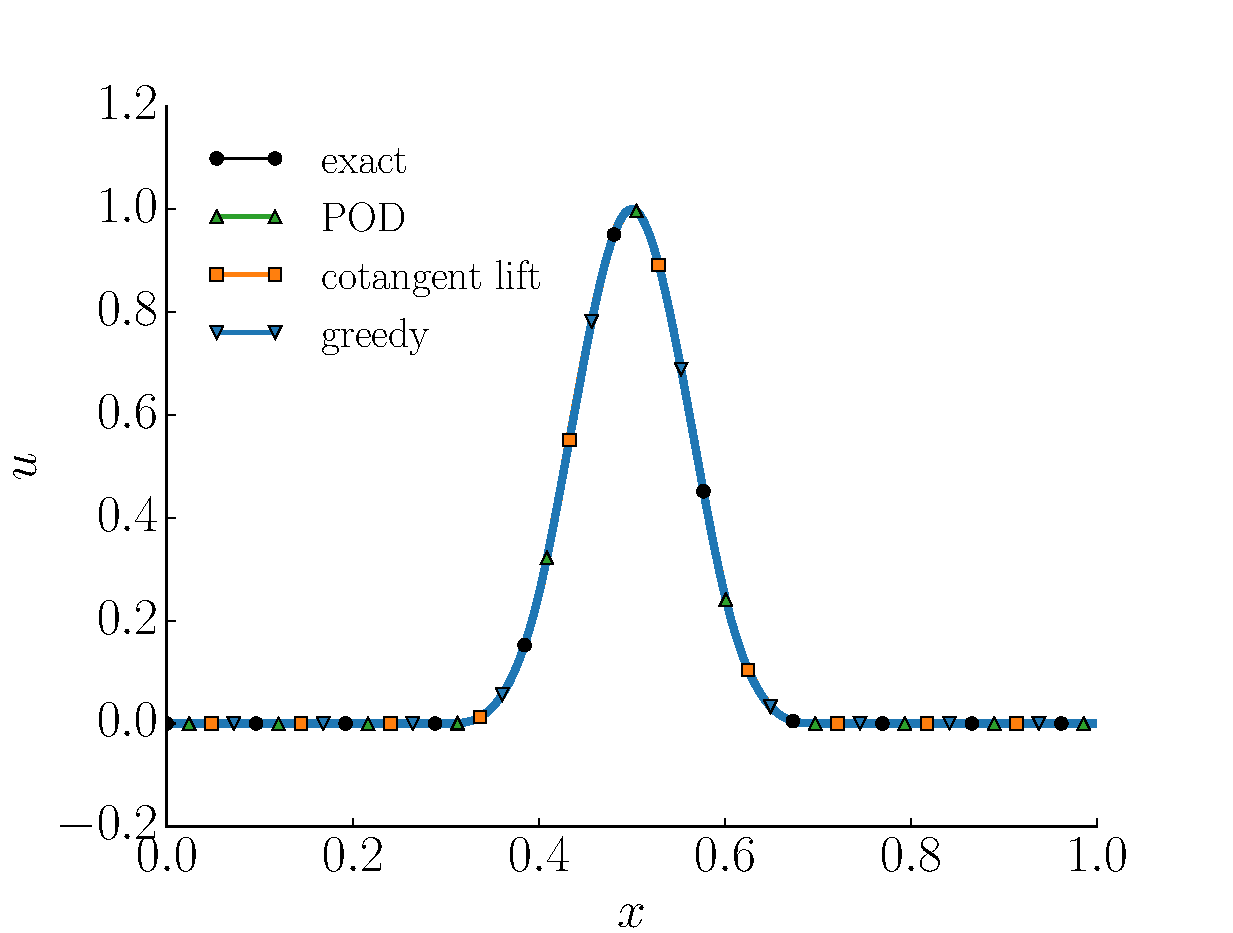
\includegraphics[width=1\textwidth]{./images/paper1/wave/solution/solution_t0}}
\end{minipage}%
\begin{minipage}{.5\linewidth}
\centering
\subfloat[$t=1$]{\label{fig:NuRe:1b}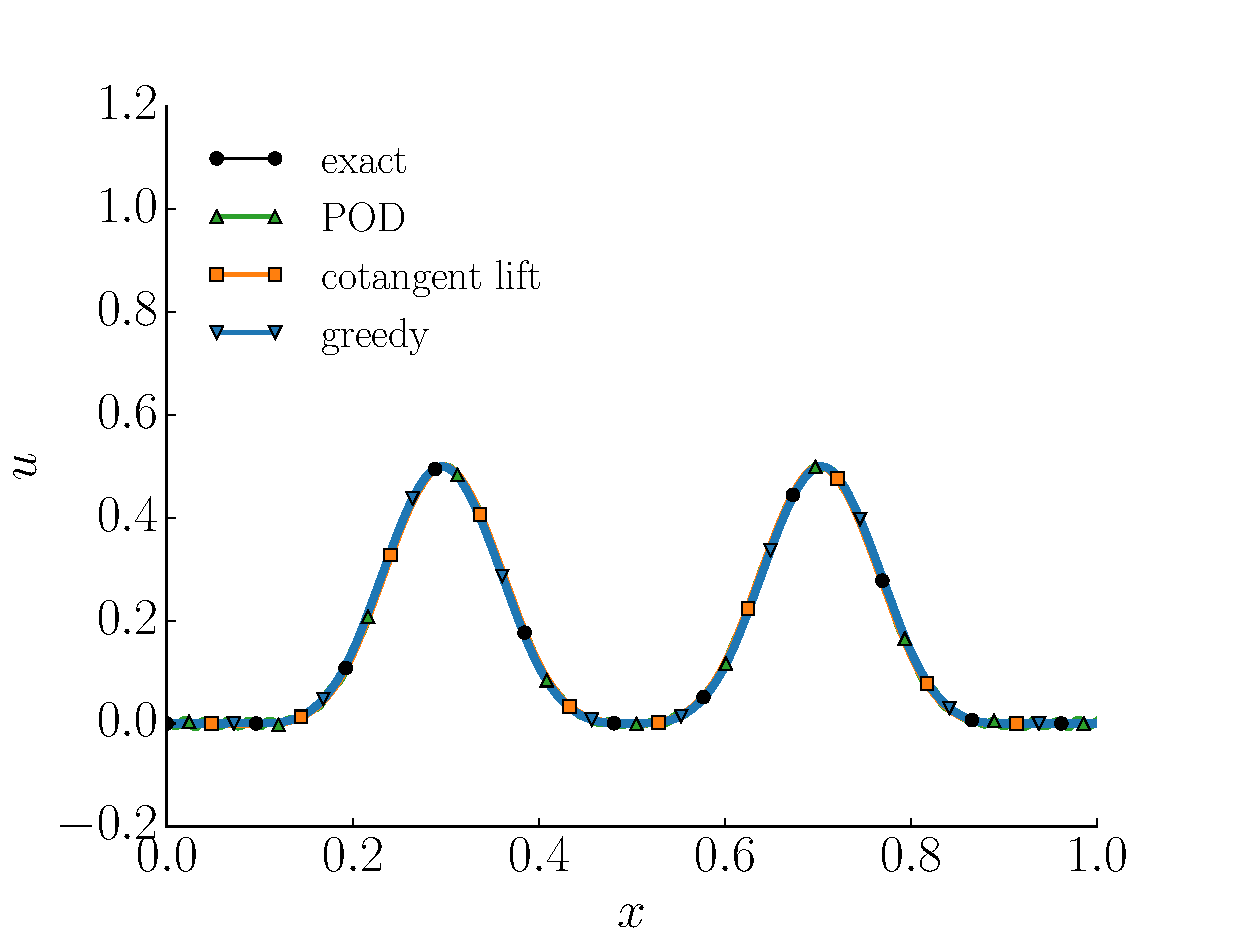
\includegraphics[width=\textwidth]{./images/paper1/wave/solution/solution_t1}}
\end{minipage}\par\medskip
\centering
\subfloat[$t=2$]{\label{fig:NuRe:1c}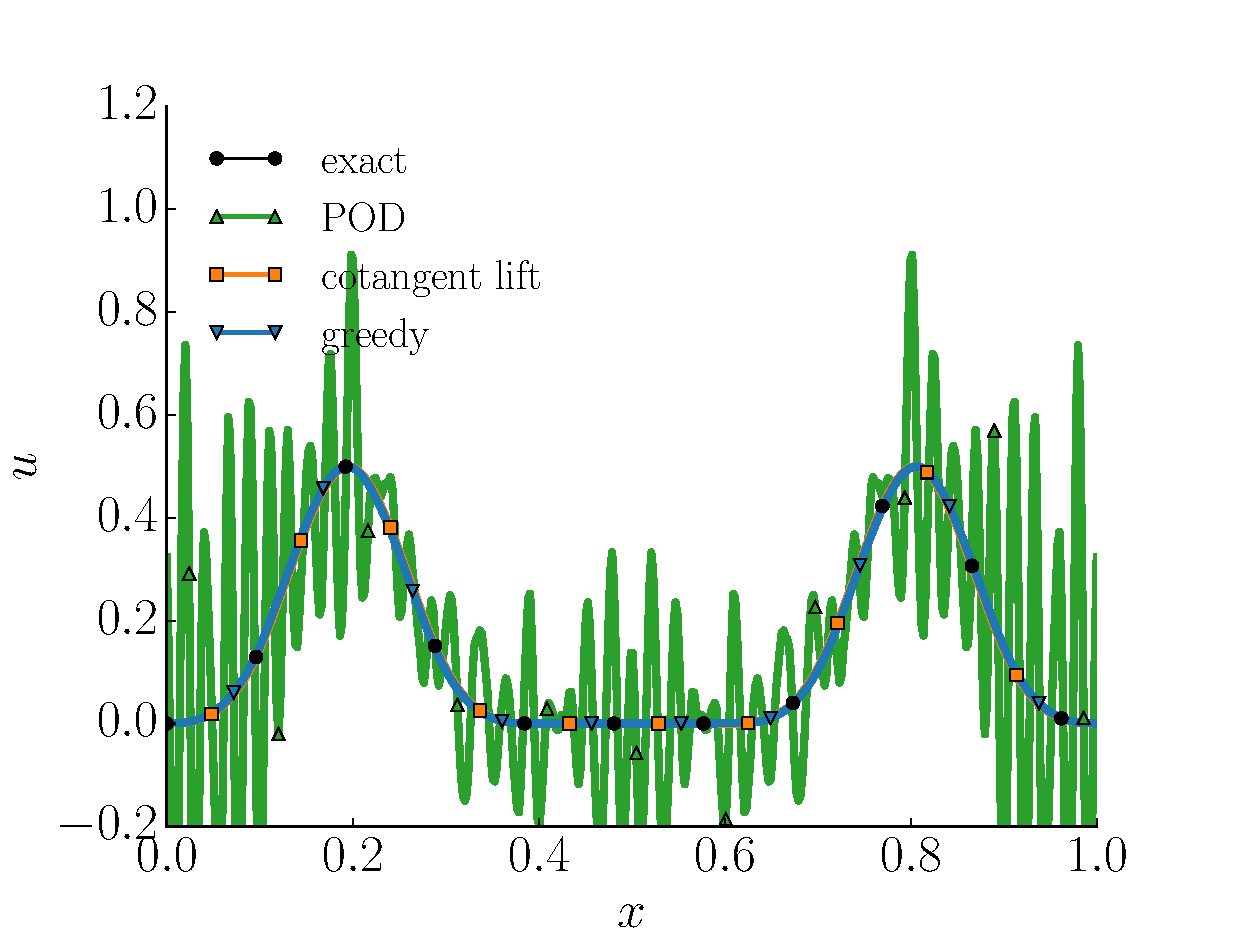
\includegraphics[width=0.5\textwidth]{./images/paper1/wave/solution/solution_t2}}
\caption{The solution $q$ at $t=0$, $t=1$ and $t=2$ of the linear wave equation for parameter value $c= 0.1019$ different from training parameters. Here, the solution of the full system together with the solution of the POD, cotangent lift, complex SVD and the greedy reduced system is shown.}
\label{fig:NuRe:1}
\end{figure}

\begin{figure}

\begin{minipage}{.5\linewidth}
\centering
\subfloat[]{\label{fig:NuRe:2c}\includegraphics[width=\textwidth]{./images/paper1/wave/error}}
\end{minipage}%
\begin{minipage}{.5\linewidth}
\centering
\subfloat[]{\label{fig:NuRe:2b}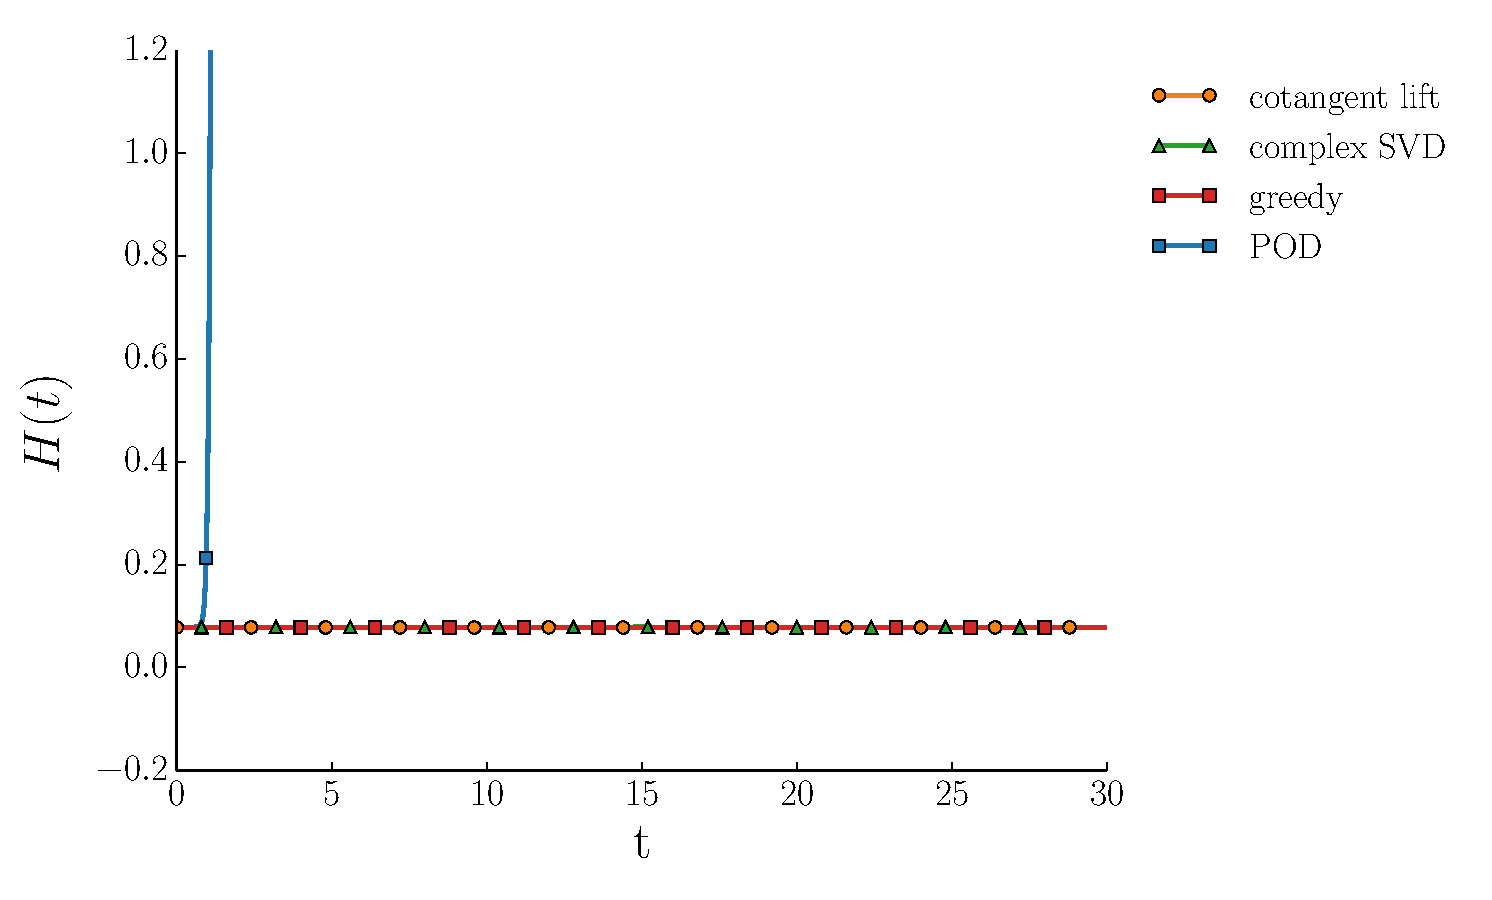
\includegraphics[width=\textwidth]{./images/paper1/wave/hamiltonian}}
\end{minipage}\par\medskip
\centering
%\subfloat[]{\label{fig:NuRe:2c}\includegraphics[width=0.5\textwidth]{./figs/wave/error}}

\caption{(a) The $L^2$-error between the solution of the full system and the reduced system for different model reduction methods for $t \in [0,30]$. (b) Plot of the Hamiltonian function for $t \in [0,30]$. }
\label{fig:NuRe:2}
\end{figure}



Figure \ref{fig:NuRe:1a} shows the solution of the linear wave equation for parameter values $(\omega_1,\omega_2,\omega_3,\omega_4) = (0.8456,0.1320,0.9328,0.5809)$ or $\kappa(\omega) = 0.1019$, chosen to be different from training parameters, at $t=0$, $t = 1$ and $t=2$. While we see instability and divergence from the exact solution for the POD reduced system, the symplectic methods provide a good approximation of the full model. 

The decay of the singular values for the POD are shown in Figure \ref{fig:NuRe:5a}. The decay of the singular values suggests that a low dimensional solution manifold indeed exists. However, since the linear subspace, constructed by the POD, is not symplectic, we observe blow up of the Hamiltonian function in Figure \ref{fig:NuRe:2b} and the instability of the solution in Figure \ref{fig:NuRe:1}. The symplectic methods (using a reduced basis of the same size as POD) preserve the Hamiltonian function as shown in Figure \ref{fig:NuRe:2b}.

Figure \ref{fig:NuRe:2c} shows the $L^2$-error between the solution of the full model and the reduced systems constructed by different methods. We note that the error for the POD reduced system rapidly increases, confirming that the projection based reduced system does not yield a stable solution. Furthermore, the symplectic methods provide a better approximation since the geometric structure of the original system is preserved. Although the greedy method is almost twice faster than the SVD-based methods in the offline stage, its accuracy is comparable. The cotangent lift method provides a more accurate solution, on the other hand the cotangent lift basis (\ref{p1.eq:SyMo:9}) takes a less general form and usually computationally more demanding than the greedy method.

For complex systems were the solution of the full system is expensive and for high dimensional parameter domains, POD-based methods become impractical \cite{hesthaven2015certified,quarteroni2015reduced}. However, the greedy method requires substantially fewer (proportional to the size of the reduced basis) evaluation of the time integration of the original system.

\subsection{Nonlinear Schr\"odinger Equation} \label{chap:NuRe:1.2} Let us consider the one-dimensional parametric Schr\"odinger equation
\begin{equation} \label{eq:NuRe:10}
\left\{
\begin{aligned}
	& i u_t(t,x,\epsilon) = - u_{xx}(t,x,\epsilon) - \epsilon |u(t,x,\epsilon)|^2 u(t,x,\epsilon),\\
	& u(0,x) = u_0(x),
\end{aligned}
\right.
\end{equation}
where $u$ is a complex valued wave function, $i$ is the imaginary unit, $|\cdot|$ is the modulus operator and $\epsilon$ is a parameter that belongs to the interval $\Gamma = [0.9,1.1]$. We consider periodic boundary conditions, i.e., $x$ belongs to a one-dimensional torus of length $L$. We consider the initial condition
\begin{equation} \label{eq:NuRe:11}
	u_0(x) = \frac{\sqrt 2}{\cosh(x - x_0)} \exp(i\frac{c(x-x_0)}{2}),
\end{equation}
for a positive constant $c$. In quantum mechanics, the quantity $|u(t,x)|^2$ represents the probability of finding the system in state $x$ at time $t$. For the choice of $\epsilon = 1$, $|u(x,t)|$ becomes a solitary wave, and the initial condition will be transported in the positive $x$ direction with a constant speed. For other choices of $\epsilon$, the solution comprises an ensemble of solitary waves, moving in either direction \cite{faou2012geometric}. 

By introducing the real and imaginary variables $u = p + iq$, we can rewrite (\ref{eq:NuRe:10}) in canonical form as
\begin{equation} \label{eq:NuRe:12}
\left\{
\begin{aligned}
 q_t &= p_{xx} + \epsilon (q^2+p^2)p, \\
 p_t &= -q_{xx} - \epsilon (q^2 + p^2)q,
\end{aligned}
\right.
\end{equation}
with the Hamiltonian function
\begin{equation} \label{eq:NuRe:13}
	H(q,p) = \int_{0}^{L} (q_x^2 + p_x^2) + \frac \epsilon 2 (q^2 + p^2)^2\ dx.
\end{equation}
We discretize the torus into $N$ equidistant points and take $\Delta x = L/N$, $x_i = i\Delta x$, $q_i=q(t,x_i,\epsilon)$ and $p_i = p(t,x_i,\omega)$ for $i = 1 ,\dots,N$. A central finite differences scheme is used to discretize (\ref{eq:NuRe:12}) as
\begin{equation}  \label{eq:NuRe:14}
	\frac{d}{dt} z = \mathbb J_{2N} Lz + \mathbb J_{2N} g(z).
\end{equation}
Here $z = (q_1,\dots,q_N,p_1,\dots,p_n)^T$ and
\begin{equation}  \label{eq:NuRe:15}
	L = 
	\begin{pmatrix}
		D_{xx} & 0_N \\
		0_N & D_{xx}
	\end{pmatrix}.
\end{equation}
Here $\mathbf g$ is a vector valued nonlinear function defined as
\begin{equation}  \label{eq:NuRe:16}
	\mathbf g(\mathbf z) =
	\begin{pmatrix}
	(q_1^2 + p_1^2)q_1 \\
	\vdots \\
	(q_N^2 + p_N^2)q_N \\
	(q_1^2 + p_1^2)p_1 \\
	\vdots \\
	(q_N^2 + p_N^2)p_N
	\end{pmatrix}.
\end{equation}
We discretize the Hamiltonian to obtain
\begin{equation}  \label{eq:NuRe:17}
	H_{\Delta x}(\mathbf z) = {\Delta x}\sum_{i=1}^{N} \left( \frac{q_i q_{i-1} - q_i^2}{\Delta x ^2} + \frac{p_i p_{i-1} - p_i^2}{\Delta x ^2} + \frac \epsilon 4 (p_i^2 + q_i^2)^2  \right),
\end{equation}
and use a St\"ormer-Verlet (\ref{eq:2.23}) scheme for time integration. Since the Hamiltonian function (\ref{eq:NuRe:17}) is non-separable, this scheme is implicit, therefore, in each time iteration, a system of nonlinear equations is solved using Newton's iteration. We summarize the physical and numerical parameters for the full model in the following table

\vspace{0.5cm}
\begin{center}
\begin{tabular}{|l|l|}
\hline
Domain length & $L = 2\pi /l$ \\
Domain scaling factor & $l = 0.11$ \\
wave speed & $c =1$\\
No. grid points & $N = 256$ \\
Space discretization size & $\Delta x = 0.2231$ \\
Time discretization size & $\Delta t = 0.01$ \\
\hline
\end{tabular}
\end{center}
\vspace{0.5cm}
Regarding computation of the nonlinear terms of reduced systems, we compare the DEIM with the symplectic DEIM. For generation of the DEIM reduced basis we apply \Cref{alg:3.4} to the set of nonlinear snapshots. The method discussed in \Cref{sec:3.6} is used to construct a reduced basis appropriate for the symplectic DEIM. The tolerance for the projection error is set to $\delta = 10^{-4}$.

We compare the reduced system obtained using the greedy algorithm with the cotangent lift, the complex SVD, DEIM, the symplectic DEIM and also the POD. For the SVD-based methods, we discretize the parameter space $[0.9,1.1]$ into $M=500$ equidistant grid points across the discrete parameter space $\Gamma_M = \{\epsilon_1,\dots,\epsilon_M \}$, and gather trajectory snapshots for each $\epsilon_i$ for $i = 1,\dots,M$ in the snapshots matrix $S$. All reduced systems are taken to have identical sizes ($k=90$ for the symplectic methods and $k=180$ for the POD method). Following \Cref{alg:4.1} we construct the reduced system using the same discrete parameter space $\Gamma_M$. The tolerance for the error in the Hamiltonian is set to $\delta = 10^{-3}$. Moreover, for DEIM and symplectic DEIM, we construct bases of size $k'=80$. Note that the reduced system, generated in the symplectic DEIM, will be of size $k+k'=170$.

The cost of the offline stage is reduced to 20\% when using the greedy method for constructing a symplectic basis of size $k=90$, as compared to the SVD-based methods. The online stage, i.e., time integration for a new parameter in $\Gamma$, is generally more than 3 times faster than for the original system. We point out that the efficiency of reduced systems are implementation and platform dependent and we expect further reduction as the size of the problem increases.
  
\begin{figure}

\begin{minipage}{.5\linewidth}
\centering
\subfloat[$t=0$]{\label{fig:NuRe:3a}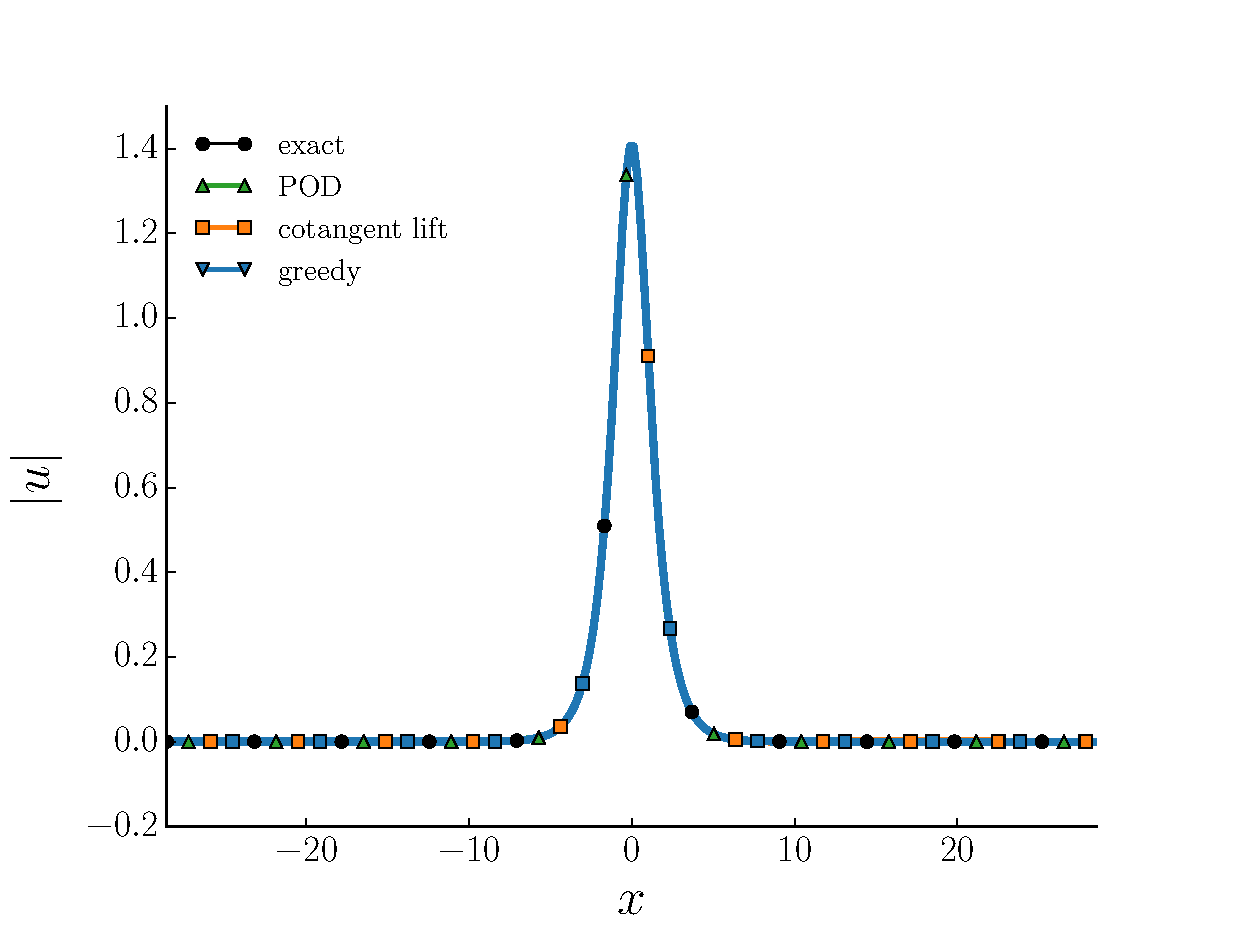
\includegraphics[width=1\textwidth]{./images/paper1/schrodinger/solution/solution_t0}}
\end{minipage}%
\begin{minipage}{.5\linewidth}
\centering
\subfloat[$t=10$]{\label{fig:NuRe:3b}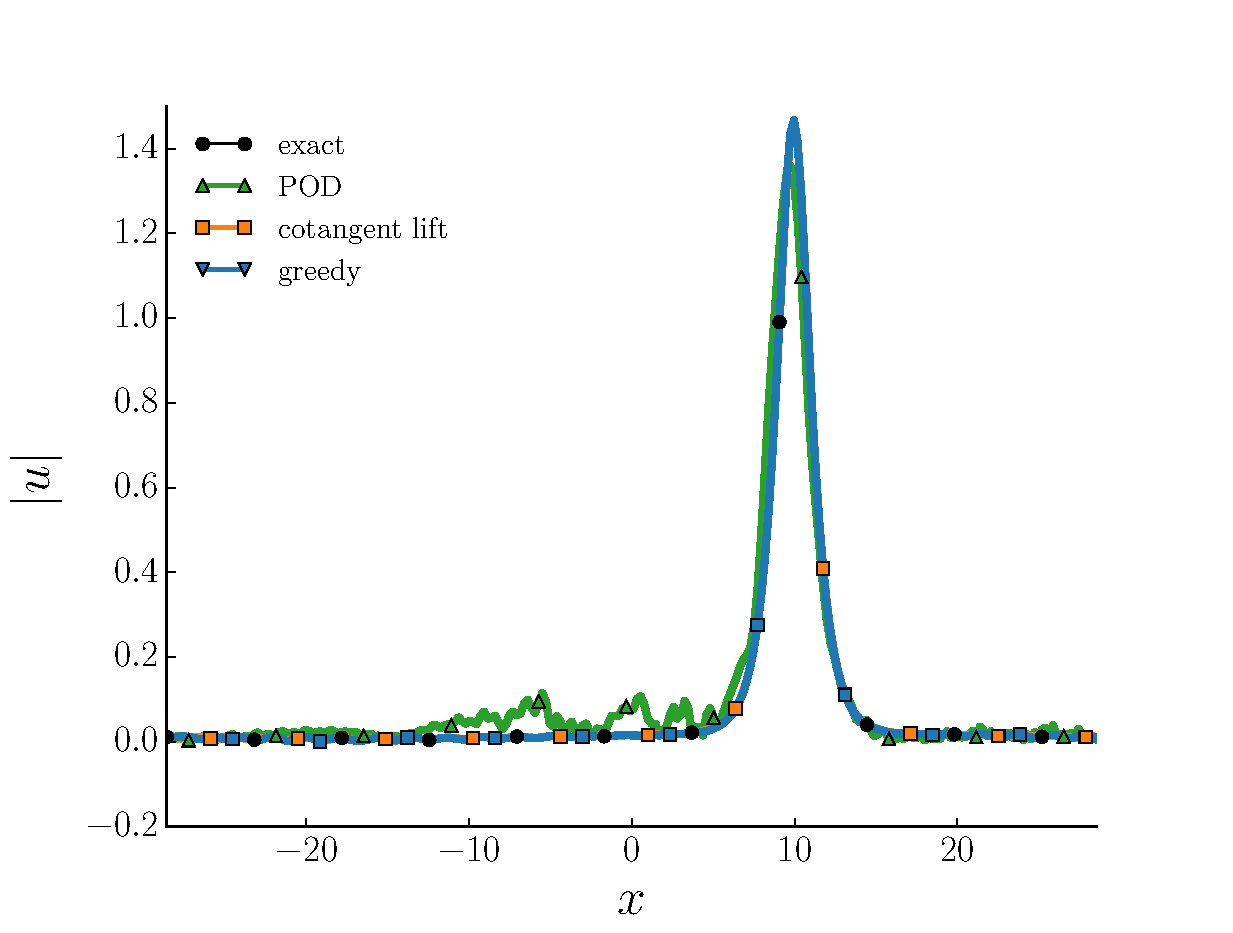
\includegraphics[width=\textwidth]{./images/paper1/schrodinger/solution/solution_t10}}
\end{minipage}\par\medskip
\centering
\subfloat[$t=20$]{\label{fig:NuRe:3c}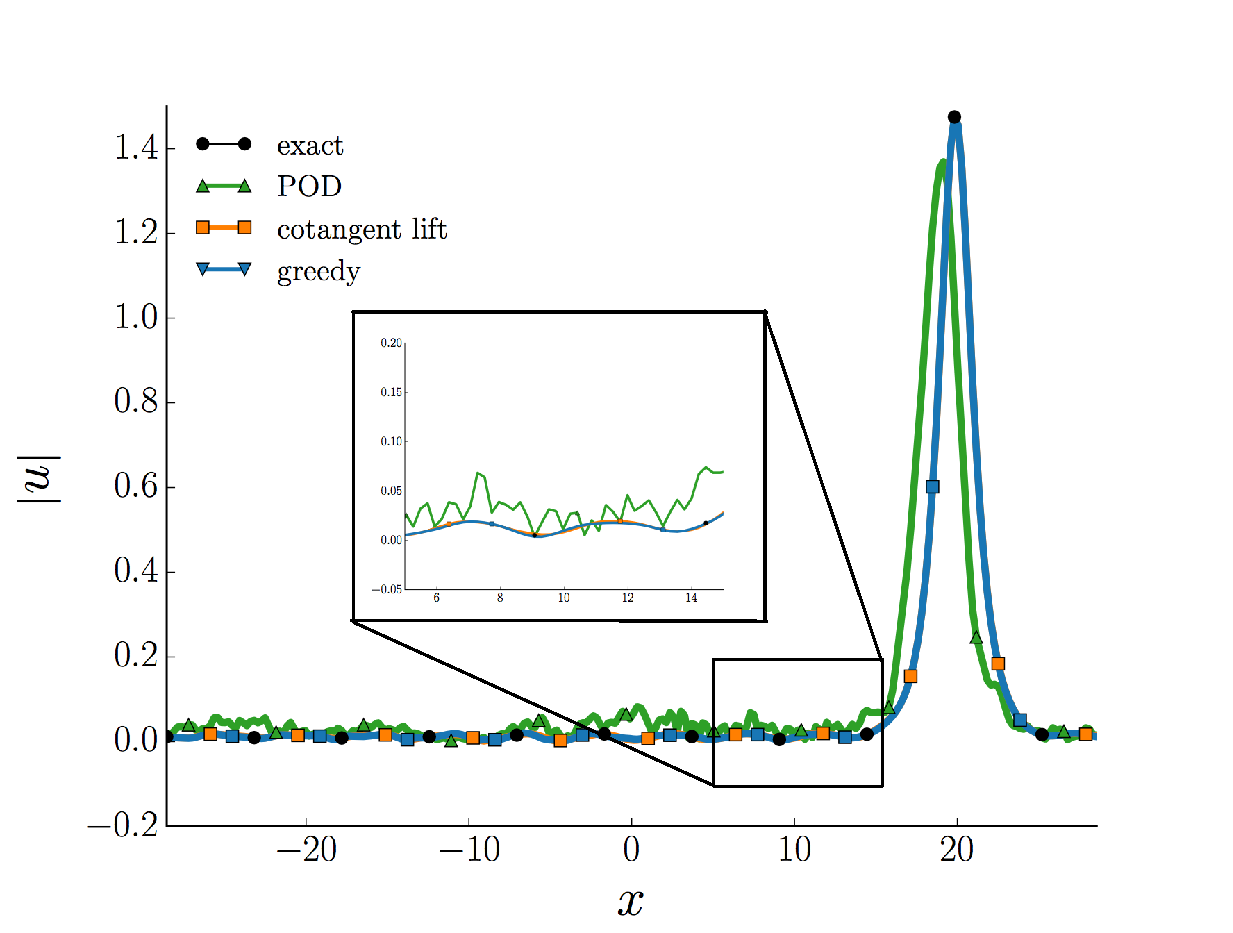
\includegraphics[width=0.5\textwidth]{./images/paper1/schrodinger/solution/solution_t20}}
\caption{The solution $|u(t,x)| = \sqrt{q^2 + p^2}$ at $t=0$, $t=10$ and $t=20$ of the Nonlinear Schr\"odinger equation for parameter value $\epsilon = 1.0932$. Here the solution of the full system, together with the solution of the POD, cotangent lift, complex SVD and the greedy reduced system, is shown.}
\label{fig:NuRe:3}
\end{figure}

\begin{figure}

\begin{minipage}{.5\linewidth}
\centering
\subfloat[]{\label{fig:NuRe:4c}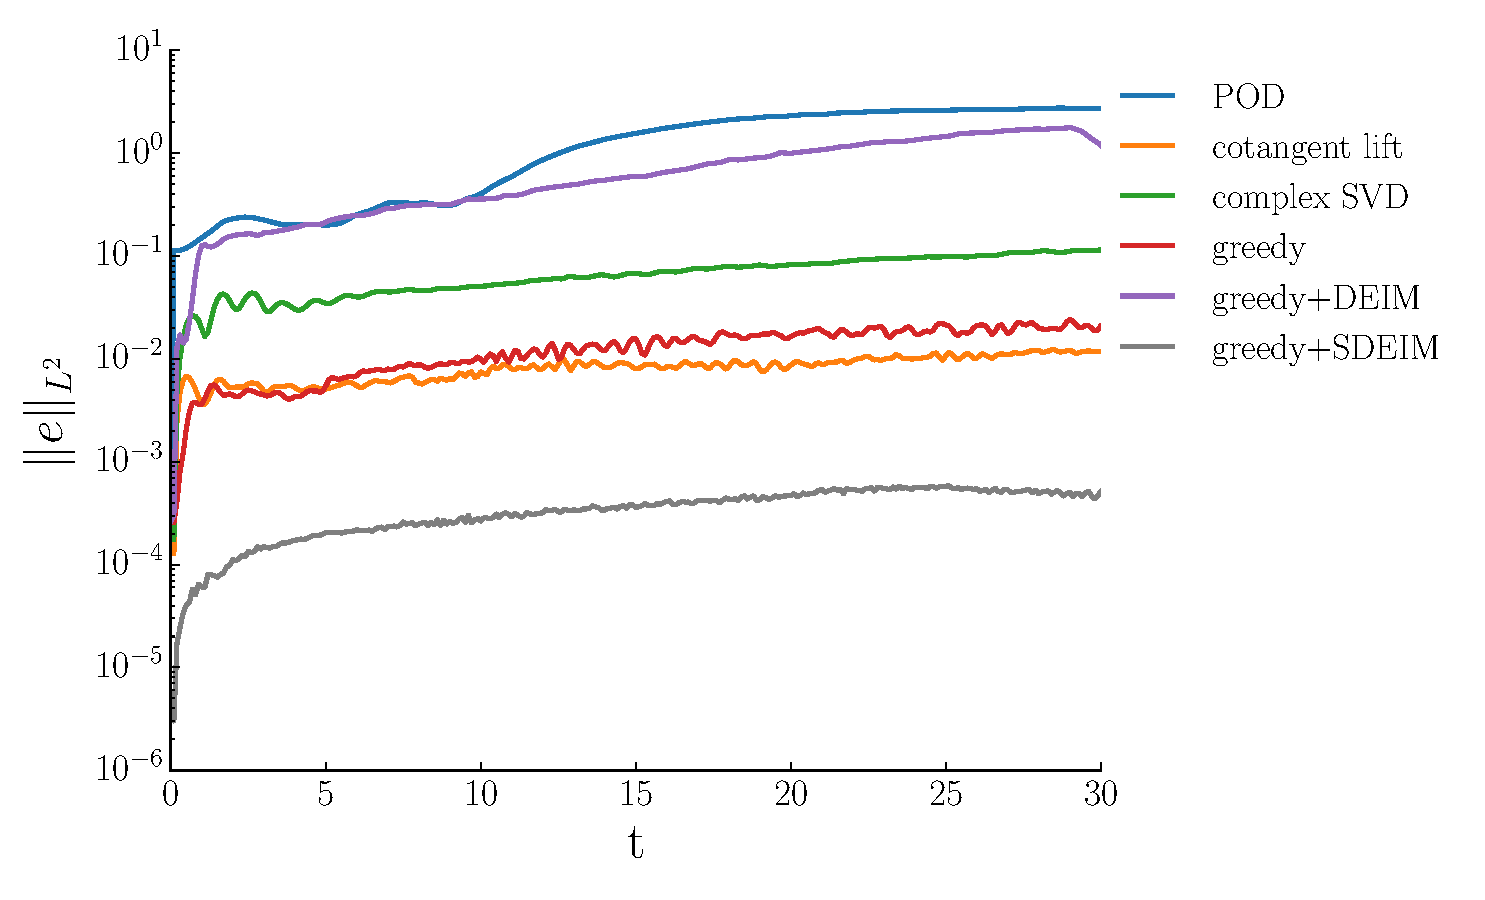
\includegraphics[width=\textwidth]{./images/paper1/schrodinger/error}}
\end{minipage}%
\begin{minipage}{.5\linewidth}
\centering
\subfloat[]{\label{fig:NuRe:4b}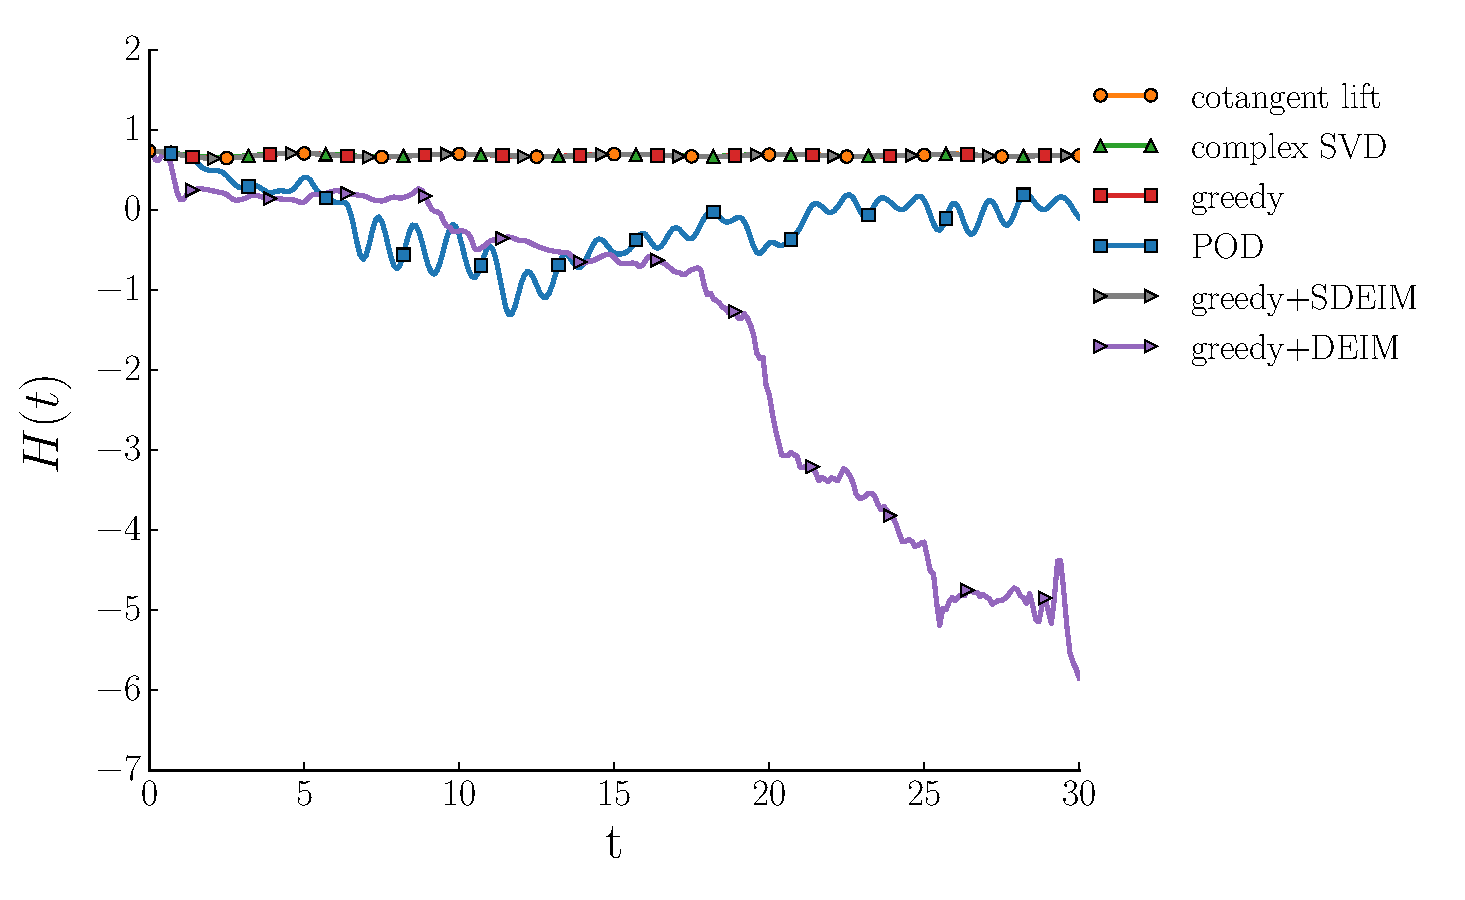
\includegraphics[width=\textwidth]{./images/paper1/schrodinger/hamiltonian}}
\end{minipage}\par\medskip
\centering
%\subfloat[]{\label{fig:NuRe:4c}\includegraphics[width=0.5\textwidth]{./figs/schrodinger/error}}

\caption{ (a) Plot of the Hamiltonian function for $t \in [0,30]$. (b) The $L^2$ error between the solution of the full system and the reduced system for different model reduction methods for $t \in [0,30]$. }
\label{fig:NuRe:4}
\end{figure}


Figure \ref{fig:NuRe:3} shows the solution of the Schr\"odinger equation for parameter value $\epsilon = 1.0932$ at $t=0$, $t=10$ and $t=20$. We first compare the reduced system obtained by the greedy algorithm with the POD, the cotangent lift, and the complex SVD method. The size of the reduced systems are taken identical for all methods ($k=180$ for POD and $k=90$ for the rest). Although the decay of the singular values in Figure \ref{fig:NuRe:5b} suggests that the accuracy of the POD reduced system should be comparable to that of the other methods, we observe instabilities in the solution at $t=10$. The greedy, the cotangent lift and the complex SVD method, on the other hand, generate a stable reduced system that accurately approximates the solution of the full model.

In Figure \ref{fig:NuRe:4b} we observe that the symplectic methods preserve the Hamiltonian function, unlike the POD and the DEIM methods. We emphasise that using the reduced basis, obtained by the greedy, together with the DEIM (purple line) does not preserve the symplectic structure as suggested in this figure.

Figure \ref{fig:NuRe:4c} illustrates the $L^2$-error between the solution of the full model with the reduced systems, generated by different methods. We first observe that symplectic methods yield a lower computational error when compared to non-symplectic methods. Secondly, we observe that although the reduced systems from the cotangent lift and the complex SVD are of the same size, their accuracy is different by an order of magnitude. We notice that the greedy algorithm is slightly less accurate than the cotangent lift method while its offline computational cost is reduced to 20\% when compared to the cotangent lift. Lastly we notice that the combination of the greedy reduced basis and DEIM yields large errors in the solution while the solution using the symplectic DEIM is very accurate. We note that the symplectic DEIM is even more accurate than the greedy itself since it has been enriched by the nonlinear snapshots. 

\subsection{Numerical Convergence} In this section we discuss the numerical convergence of the symplectic greedy method introduced in Section \ref{chap:SyMo:1}. The exponential convergence properties of the conventional greedy \cite{Quarteroni:2016wi} is presented in \cite{Buffa:2012iz,Binev:2011fj}. Theorem \ref{theorem:SyMo:2} suggests that the symplectic greedy method has similar properties. To illustrate this we compare the convergence of the conventional greedy with the convergence of the symplectic greedy method through the numerical simulations in Sections \ref{chap:NuRe:1.1} and \ref{chap:NuRe:1.2}. 

The decay of the singular values of the snapshot matrix for the parametric wave equation and the nonlinear Schr\"odinger equation are given in Figure \ref{fig:NuRe:5}. The decay rate of the singular values is a strong indicator for the decay rate of the Kolmogorov $n$-width of the solution manifold. We expect that the conventional greedy method and the symplectic greedy method provide a similar rate in the decay of the error.
	
Figure \ref{fig:NuRe:5} shows the maximum $L^2$ error between the original system and the reduced system at each iteration of different greedy methods. In this figure we find the conventional greedy with orthogonal projection error as a basis selection criterion (orange), the symplectic greedy method with a symplectic projection error as a basis selection criterion (green), and the symplectic greedy method with energy loss $\Delta H$ as a basis selection criterion (red).

It is observed that the decay rate of the error for greedy with the orthogonal projection and the greedy with the symplectic projection is similar to the decay of the singular values. This matches our expectation from Theorem \ref{theorem:SyMo:2}. We also notice that the greedy method with the loss in Hamiltonian provides an excellent error indication as a basis selection criterion.


\begin{figure}

\begin{minipage}{.5\linewidth}
\centering
\subfloat[]{\label{fig:NuRe:5a}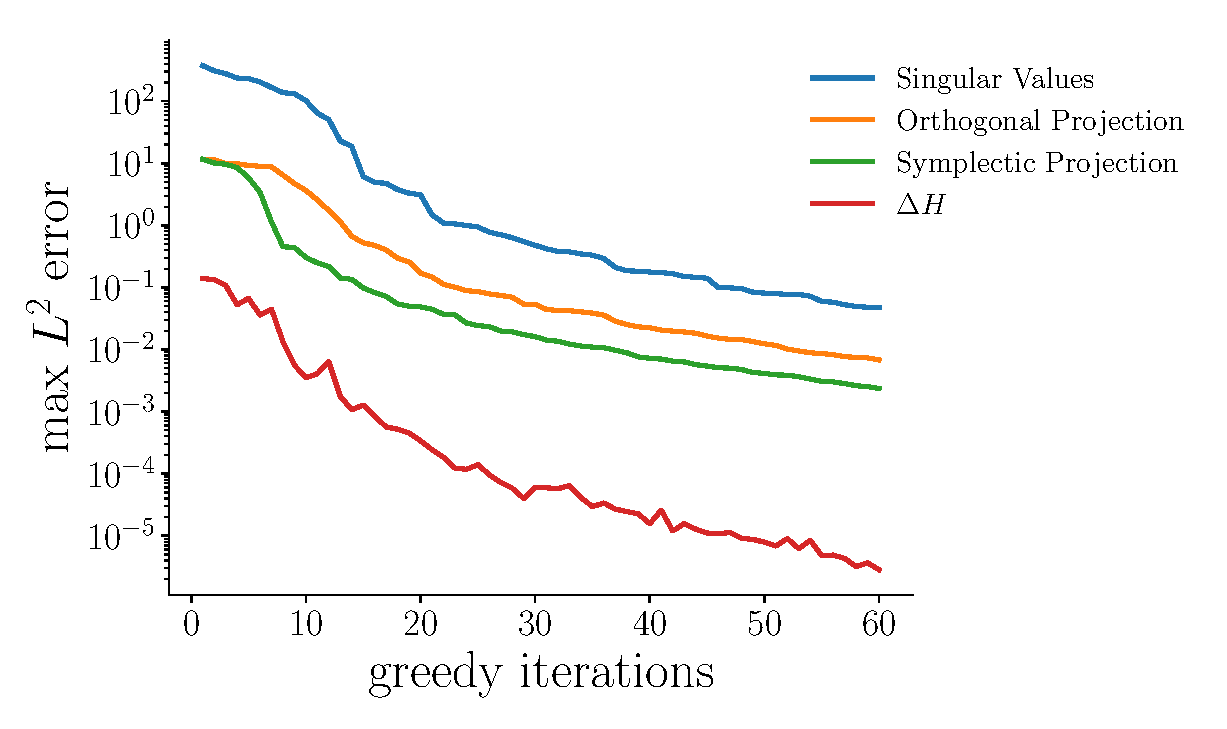
\includegraphics[width=\textwidth]{./images/paper1/wave/convergence}}
\end{minipage}%
\begin{minipage}{.5\linewidth}
\centering
\subfloat[]{\label{fig:NuRe:5b}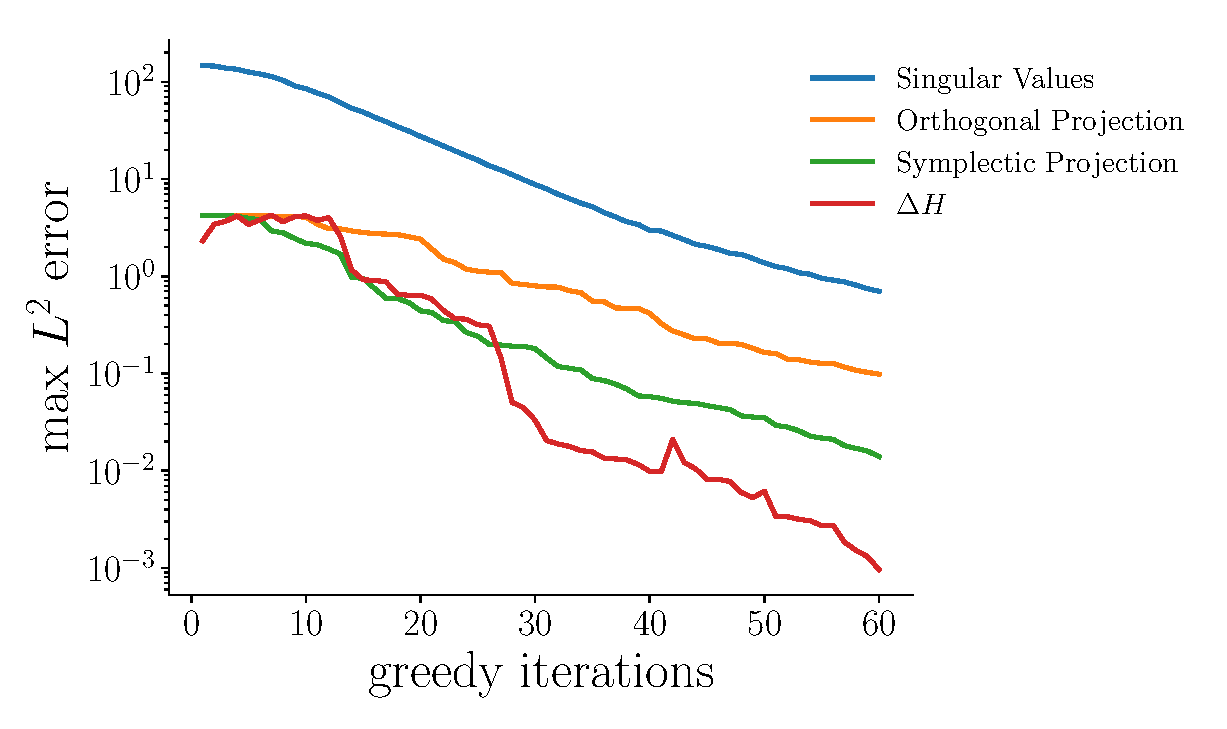
\includegraphics[width=\textwidth]{./images/paper1/schrodinger/convergence}}
\end{minipage}\par\medskip
\centering
%\subfloat[]{\label{fig:NuRe:4c}\includegraphics[width=0.5\textwidth]{./figs/schrodinger/error}}

\caption{ (a) Convergence of the greedy method for the wave equation. (b) Convergence of the greedy method for the nonlinear Schr\"odinger equation equation. }
\label{fig:NuRe:5}
\end{figure}

\section{Conclusion} \label{chap:Con:1}

In this paper, we present a greedy approach for the construction of a reduced system that preserves the geometric structure of Hamiltonian systems. An iteration of the greedy method comprises searching the parameter space using the error in the Hamiltonian, to find the best basis vectors that increase the overall accuracy of the reduced basis. We argue that for a compact subset with exponentially small Kolmogorov $n$-width we recover exponentially fast convergence of the greedy algorithm. For fast approximation of nonlinear terms, the basis obtained by the greedy was combined with a symplectic DEIM to construct a reduced system with a Hamiltonian that is arbitrary close to the Hamiltonian of the original system.

The numerical results demonstrate that the greedy method can save substantial computational cost in the offline stage as compared to alternative SVD-based techniques. Also since the reduced system obtained by the greedy method is Hamiltonian, the greedy method yields a stable reduced system. Symplectic DEIM effectively reduces computational cost of approximating nonlinear terms while preserving stability and symplectic structure. Hence, the greedy method is an efficient model reduction technique that provides an accurate and stable reduced system for large-scale parametric Hamiltonian systems.

\section*{Acknowledgments}
We would like to thank the referees for providing us with very useful comments which served to improve the paper.


